%%%%%%%%%%%%%%%%%%%%%%%%%%%%%%%%%%%
%%%  Filename: thesis_template.tex
%%%  ---
%%%  Template for Master Thesis at DTETI UGM   		
%%%  Created using thesisdtetiugm.cls
%%%  --- 
%%%  Written by Canggih Puspo Wibowo
%%%  [canggihpw@gmail.com]
%%%%%%%%%%%%%%%%%%%%%%%%%%%%%%%%%%%

%% Use option "bahasa" or "english" 
%%    to change the basic language used
%% User option "bachelor", "master", or "doctoral"
%% 	  to change the degree
% \documentclass[<bachelor/master/doctoral>,<bahasa/english>]{thesisdtetiugm}
\documentclass[bachelor,bahasa]{thesisdtetiugm}
%======================================
% Information Input
%======================================
% Input author's name and ID number
\author{Muhamad Alif Ridha}{19/439613/TK/48343}
% Input the thesis' title
\title{Pengaruh Jumlah \textit{Hidden Layer} terhadap Kinerja Akurasi dan Waktu Pembelajaran pada Jaringan Syaraf Tiruan}
% Program and the head of the program
\program{Teknik Elektro}{Ir. Adha Imam Cahyadi, S.T., M.Eng., D.Eng., IPM.}{197902112008121001}
% Name of department head and NIP
\departmenthead{Ir. Hanung Adi Nugroho, S.T., M.E., Ph.D., IPM.}{1978 0224 2002 12 1 001}
\major{Teknik Elektro}
\yearsubmit{2023}
\examdate{<<Exam date>>}
% Name of thesis supervisors/promotors
\addsupervisor{Dr. Ir. Risanuri Hidayat, M.Sc.}{<<NIP xxxxxx>>}
\addsupervisor{Prof. Dr. Ir. Sasongko Pramono Hadi, DEA.}{<<NIP xxxxxx>>}
%\addsupervisor{<<Supervisor 3>>}{<<NIP>>}
% Name of examiners
%\addexaminer{<<Examiner 1>>}{<<NIP 1>>}
%\addexaminer{<<Examiner 2>>}{<<NIP 2>>}
%\addexaminer{<<Examiner 3>>}{<<NIP 3>>}
%\addexaminer{<<Examiner 4>>}{<<NIP 4>>}
%\addexaminer{<<Examiner 5>>}{<<NIP 5>>}
%\addexaminer{<<Examiner 6>>}{<<NIP 6>>}
%\addexaminer{<<Examiner 7>>}{<<NIP 7>>}
%\addexaminer{<<Examiner 8>>}{<<NIP 8>>}
%\addexaminer{<<Examiner 9>>}{<<NIP 9>>}

%======================================

% correct bad hyphenation here [example]
% \babelhyphenation[<<english/bahasa>>]{op-tical net-works semi-conduc-tor}
%% Uncomment block of code below to disable hyphenation
%\tolerance=1
%\emergencystretch=\maxdimen
%\hyphenpenalty=10000
%\hbadness=10000

\begin{document}
%======================================
% Create cover etc
%======================================

%---- COVER ----
%\printcover{sample/logougm.png}{Pendadaran/Tesis/Ringkasan Tesis*}
\printcover{sample/logougm.png}{Bachelor}
% *Choose one

%---- ENDORSEMENT PAGE ----
% Select endorsement page type. If you want to use your own PDF file,  
% 	use \printendorsementpdf, or if you want to use JPG file, use 
% 	\printendorsementjpg. Otherwise, use \printendorsement.
% 	Choose one only. Comment out unused command(s).
%
%\printendorsement
%\printendorsementpdf

%\printendorsementjpg{sample/scanned-endorsement.jpg}

%---- DEDICATION PAGE ----
%\chapterstatement{contents/statement/statement}
%\chapterstatementjpg

\chapterdedication{contents/dedication/dedication}

%---- STATEMENT PAGE ----
% Select statement page type. If you want to use your own JPG file,  
%	use \chapterstatementjpg{<your *.jpg file path>}. Otherwise, 
%	use \chapterstatement{contents/statement/statement}.
%	Choose one only. Comment out unused command(s).
%


%---- PREFACE PAGE ----
 \chapterpreface{contents/preface/preface}

%======================================
% Create Table of Contents, List of Figures, List of Tables
% <Do not change this part>
%======================================
\cleardoublepage 
\phantomsection
\thetoc
\onehalfspacing
\tableofcontents
\singlespacing
\cleardoublepage 
\phantomsection
\thelot
\listoftables
\cleardoublepage \phantomsection \thelof
\listoffigures

%======================================

%---- NOMENCLATURE PAGE ----
\chapternomenclature{contents/nomenclature/nomenclature}

%---- INTISARI PAGE----
\chapterintisari{contents/abstract/intisari}

%---- ABSTRACT PAGE----
\chapterabstract{contents/abstract/abstract}


%======================================



%======================================
%  MAIN TEXT
%======================================
\startmain
% You can change 
%    the filename and location of the files inputted
\chapter{Pendahuluan}

\section{Latar Belakang}

Belakangan ini penggunaan kecerdasan artifisial (KA) semakin berkembang dan menjadi perhatian global. Data dari laporan terbaru menunjukkan bahwa investasi global dalam teknologi KA terus meningkat, dengan perkiraan mencapai lebih dari 300 miliar dolar AS pada tahun 2023\cite{300mn}. Perusahaan-perusahaan besar seperti Google, Amazon, dan Facebook ikut mengintegrasikan KA ke dalam produk dan layanan mereka untuk meningkatkan efisiensi dan pengalaman pengguna\cite{Kelleher2019-cj}. Selain itu, KA juga telah merambah ke berbagai sektor, termasuk kesehatan, keuangan, otomotif, dan manufaktur. Misalnya, dalam industri kesehatan, KA digunakan untuk menganalisis data medis dan membantu dalam diagnosis penyakit\cite{Early_Diagnosis_of_Alzheimer's_Disease}. Di sektor keuangan, KA digunakan untuk mengoptimalkan portofolio investasi dan mendeteksi keadaan obligasi dimasa depan. 

Indonesia pun tidak ingin melewatkan kesempatan ini, melalui Badan Pengkajian dan Penerapan Teknologi (BPPT). Indonesia membentuk Strategi Nasional Kecerdasan Artifisial Indonesia 2020 - 2045 (STRANAS KA)\cite{Stranaska}. Pembentukan STRANAS KA ini merupakan perwujudan Visi Indonesia Emas 2045. Untuk itu pengembangan kecerdasan artifisial akan dikaji dan diteliti untuk mengembangkan sektor-sektor yang sedang diprioritaskan. Saat ini metode kecerdasan artifisial yang sedang ramai digunakan dan dikembangkan adalah Jaringan Syaraf Tiruan (JST).

Jaringan syaraf tiruan menjadi sorotan utama dalam perkembangan kecerdasan artifisial. Model-model jaringan syaraf tiruan telah menjadi fondasi bagi berbagai aplikasi KA, seperti pengenalan wajah, penerjemah bahasa, dan \textit{driver assistance system}\cite{Auto_driving}. Keberhasilan jaringan syaraf tiruan dalam menangani tugas-tugas kompleks ini dapat dilihat dari peningkatan akurasi dan kecepatan dalam pengolahan data. Hal ini didukung dengan semakin berkembangnya teknologi yang membuat daya komputasi menjadi lebih baik dan meningkatnya penggunaan \textit{cloud} sehingga semakin memudahkan pengumpulan data dan mengurangi resiko kehilangan data. 

Secara garis besar jaringan syaraf tiruan adalah model matematis yang terdiri dari serangkaian \textit{neuron} yang terhubung satu sama lain. Setiap lapisan dalam jaringan memiliki peran khusus dalam pengolahan informasi. Salah satunya adalah \textit{hidden layer} yang bertanggung jawab untuk mengekstraksi dan mempelajari fitur-fitur kompleks dari data. Jumlah dan konfigurasi \textit{hidden layer} akan mempengaruhi kemampuan jaringan dalam memahami dan memodelkan pola dalam data. Dengan konfigurasi \textit{hidden layer} yang tepat, jaringan syaraf tiruan dapat meningkatkan kinerja dan efisiensi dalam berbagai tugas klasifikasi maupun regresi.

Salah satu permasalahan yang sering dihadapi dalam penggunaan jaringan syaraf tiruan adalah penentuan jumlah \textit{hidden layer} yang akan digunakan. Penentuan jumlah dan ukuran \textit{hidden layer} ini tidak selalu langsung dapat terlihat didalam data. Pemilihan jumlah dan ukurannya memerlukan pengaturan yang baik untuk mendapatkan hasil yang diinginkan. Secara umum jika jumlah \textit{hidden layer} terlalu sedikit, jaringan mungkin akan gagal mempelajari representasi yang cukup kompleks dari data, sementara jika terlalu banyak, dapat terjadi \textit{overfitting}, yaitu jaringan menjadi terlalu cocok dengan data yang dilatih dan kinerjanya akan menurun jika dipertemukan dengan data baru. Oleh karena itu, menemukan jumlah \textit{hidden layer} yang tepat merupakan tantangan  dalam merancang jaringan syaraf tiruan yang efektif. 

Beberapa pendekatan, seperti penggunaan \textit{cross-validation} atau teknik optimasi seperti algoritma genetika, telah digunakan untuk membantu menentukan jumlah hidden layer yang optimal dalam suatu jaringan syaraf tiruan. Meskipun kecerdasan artifisial merupakan bidang penelitian yang masih berkembang, penelitian atas permasalahan ini diharapkan akan memperkuat kemampuan jaringan syaraf tiruan untuk menghadapi berbagai tugas pemodelan dan prediksi dengan lebih akurat dan efisien.


\section{Rumusan Masalah}

Penentuan jumlah dan ukuran \textit{hidden layer} pada suatu jaringan syaraf tiruan masih memerlukan \textit{tuning} agar mendapatkan hasil yang dinginkan. Namun efek pengurangan ataupun penambahan pada \textit{hidden layer} masih ambigu dan diperlukan penelitian lebih lanjut. Oleh karena itu, maka disusun rumusan masalah seperti berikut:

\begin{enumerate}
    \item Jumlah \textit{hidden layer} pada jaringan syaraf tiruan tidak memiliki jumlah yang pasti.
    \item Belum ada informasi mengenai efek apa yang terjadi pada pengurangan dan penambahan \textit{hidden layer} pada jaringan syaraf tiruan.
    \item Belum ada informasi mengenai perngaruh jumlah \textit{hidden layer} terhadap waktu komputasi dan akurasi.
\end{enumerate}

\section{Tujuan Penelitian}

Penelitian ini bertujuan untuk menganalisis pengaruh jumlah \textit{hidden layer} dengan melakukan variasi terhadap jumlah \textit{hidden layer} sehingga akan terlihat efek yang diberikan.

\section{Batasan Penelitian}

Batasan permasalahan pada skripsi ini adalah pada data, arsitektur yang digunakan, dan variabel pengaruh yang dianalisis. Data yang digunakan adalah data yang \textit{linearly separable} artinya data dapat dipisahkan secara linier. Data memiliki 16 \textit{instance}, 2 fitur, dan tiga kelas. Kemudian batasan pada arsitektur yang digunakan. Arsitektur yang akan digunakan adalah arsitektur \textit{Multilayer Perceptron}. Pada penelitian ini tidak akan dibahas arsitektur lain seperti \textit{Convolutional Neural Network}, \textit{Reccurent Neural Network}, dll. Kemudian pengaruh yang dianalisis difokuskan pada waktu komputasi dan akurasinya.


\section{Manfaat Penelitian}

Manfaat dari penelitian ini adalah untuk mengetahui pengaruh jumlah dan ukuran \textit{hidden layer} terhadap akurasi dan waktu komputasi. Bagi akademisi dapat digunakan untuk memahami lebih lanjut mengenai jaringan syaraf tiruan dan membuka penelitian baru terkait jaringan syaraf tiruan. Bagi praktisi dapat digunakan sebagai pedoman untuk menentukan jumlah dan ukuran \textit{hidden layer} yang akan digunakan.


\section{Sistematika Penulisan}


\noindent \textbf{BAB I PENDAHULUAN}

Pada ini dijelaskan latar belakang, rumusan masalah, batasan, tujuan, manfaat, dan sistematika penulisan.

\noindent \textbf{BAB II : TINJAUAN PUSTAKA DAN LANDASAN TEORI}

Pada bab ini dijelaskan teori dan penelitian yang digunakan sebagai acuan dalam penelitian.

\noindent \textbf{BAB III : METODOLOGI PENELETIAN}

Pada bab ini berisi tentang metodologi penelitian yang terdiri atas alat dan bahan, langkah kerja, dan alur tahapan penelitian.

\noindent \textbf{BAB IV : ANALISIS DAN PEMBAHASAN}

Pada bab ini dijelaskan hasil dari penelitian dan pembahasan pengujianya.

\noindent \textbf{BAB V : KESIMPULAN DAN SARAN}

Pada bab ini ditulis kesimpulan penelitian dan saran untuk penelitian selanjutnya.

\chapter{Tinjauan Pustaka dan Dasar Teori}

\section{Tinjauan Pustaka}

Pengujian mengenai pengaruh dari jumlah lapisan tersembunyi sudah banyak dilakukan. Berikut beberapa artikel atau jurnal terkait.

Alvin J. Surkan \cite{NeuralNetforBondRating}, pada penelitiannya membuat sebuah JST untuk memprediksi rating obligasi dari \textit{moody's or standard and poor's}, data tersebut berisi tujuh buah fitur dan 126 pola obligasi sebagai \textit{instance}. Moody's memisahkan rating obligasi menjadi tujuh kelas yaitu [Aaa, Aal, Aa2, Aa3, A1 , A2, A3]. Dimana  [Aaa] adalah kualitas tinggi, [Aa1, Aa2, Aa3] adalah kualitas menengah, dan [A1, A2, A3] adalah kualitas rendah. Neural network yang dibuat akan digunakan untuk membedakan kelas kualitas tinggi [Aaa] dan kelas kualitas rendah [A1, A2, A3]. JST dibuat dengan tiga model arsitektur. satu dari tiga model menggunakan satu lapisan tersembunyi dan dua jenis lainnya menggunakan dua lapisan tersembunyi dengan jumlah hidden neuron yang berbeda, dengan masing - masing arsitektur secara berurutan [7-14-2], [7-5-10-2], dan [7-10-5-2]. hasil menunjukan dua hidden layer lebih baik dari satu hidden layer dari akurasi yang diberikan. 

Jacques de villiers\cite{backpropagationwith1and2}, pada penelitiannya menggunakan data \textit{distribution of distribution} untuk mengetahui pengaruh variasi dari data terhadap JST satu \textit{hidden layer} dan JST dua \textit{hidden layer}. Hasil penelitian yang didapatkan adalah tidak ada peningkatan performa yang signifikan antara keduanya, rata-rata satu \textit{hidden layer} memiliki klasifikasi yang lebih baik daripada dua \textit{hidden layer}, dan pelatihan dengan dua \textit{hidden layer} lebih cepat jika neuron pada kedua \textit{hidden layer} kurang lebih sama. Sedangkan peningkatan jumlah sampel dapat memberikan akurasi yang lebih baik.

Pada penelitian\cite{Panchal2011} menggunakan \textit{Hopfield Neural Networks} dan \textit{Akaike Criterion Information} untuk pemilihan jumlah hidden layer dan jumlah neuronnya. Pemilihan parameter diharapkan dapat menghindari \textit{overfitting} dan \textit{underfitting}. Hasil yang didapatkan berupa peningkatan \textit{correct classification rate} dan penurunan galat seiring dengan penambahan jumlah lapisan tersembunyi bersamaan dengan peningkatan \textit{training time}. Penulis menekankan jika penggunaan yang membutuhkan akurasi tinggi maka peningkatan jumlah lapisan tersembunyi dapat ditambahkan dan jika pada penggunaan yang memerlukan waktu yang cepat maka satu lapisan tersembunyi sudah mencukupi.

Pada penelitian\cite{Thomas2017} dibuat jaringan syaraf tiruan dengan \textit{The Levenberg-Marquardt algorithm}. Penellitian menggunakan 10 set data yang berbeda. 9 dari 10 data set menunjukan hasil yang lebih baik dalam hal akurasi pada dua lapisan tersembunyi dibandingkan satu lapisan tersembunyi, tetapi jumlah peningkatan akurasi berbeda - beda pada tiap data set dan sangat bergantung pada data set yang digunakan.

Pada artikel\cite{Uzair} berisi hasil dari artikel - artikel yang membahas pengaruh jumlah lapisan tersembunyi terhadap \textit{time complexity} dan akurasi. Dari hasil penelitiannya sulit untuk menentukan jumlah lapisan tersembunyi yang tepat hanya dengan melihat lapisan input dan lapisan outpunya saja. Meskipun banyak metode yang dapat digunakan untuk mencari jumlah lapisan tersembunyi, namun aproksimasinya akan bergantung pada data yang digunakan. Jika akurasi yang tinggi sangat dibutuhkan maka dapat menggunakan jaringan syaraf tiruan yang \textit{deep}. Namun jika \textit{time complexity} yang diinginkan maka jaringan syaraf tiruan yang \textit{deep} tidaklah cocok. Kemudian penambahan \textit{neuron} atau lapisan tersembunyi yang berlebih dapat menyebabkan \textit{overfitting}. Oleh karena itu disarankan untuk menganalisa sampel data yang digunakan agar dapat mengaproksimasi jumlah lapisan tersembunyi.
\begin{table}[H]
    \centering
    \begin{tabular}{| p{0.5cm} | p{10em} | p{5em} | p{10em} |} 
    \hline
    \textbf{No} & \textbf{Nama Penelitian} & \textbf{Metode} & \textbf{Hasil Pembahasan} \\ [0.5ex] 
    \hline
    1 & \textit{Neural Networks For Bond Rating Improved By Multiple Hidden Layers} & \textit{Multilayer Perceptron} & Dua \textit{hidden layer} lebih baik dari satu \textit{hidden layer} dari segi akurasi yang diberikan. \\ 
    \hline
    2 & \textit{Backpropagation Neural Nets with One and Two Hidden Layers} & \textit{Multilayer Perceptron} & Tidak ada perbedaan signifikan antara satu \textit{hidden layer} dan dua \textit{hidden layer}\\
    \hline
    3 & \textit{Behaviour Analysis of \textit{Multilayer Perceptron}s with Multiple Hidden Neurons and Hidden Layers} & \textit{Multilayer Perceptron} & Peningkatan jumlah lapisan tersembunyi atau jumlah neuron tersembunyi memberikan hasil yang lebih baik.\\
    \hline
    4 & \textit{Two Hidden Layers are Usually Better than One} & \textit{Multilayer Perceptron} & Dua \textit{hidden layer} lebih unggul dari satu \textit{hidden layer} \\ 
    \hline
    \end{tabular}
\end{table}

\begin{table}[H]
    \centering
    \begin{tabular}{| p{0.5cm} | p{10em} | p{5em} | p{10em} |} 
    \hline
    5 & \textit{Effects of Hidden Layers on the Efficiency of Neural networks} & \textit{Multilayer Perceptron} & Dengan jumlah lapisan tersembunyi yang sesuai dapat mengurangi waktu pelatihan dan tetap menghasilkan akurasi yang baik. Banyak metode yang dapat digunakan untuk mengaproksimasi jumlah lapisan tersembunyi, namun hal itu tetap bergantung dengan jenis data. \\ [1ex] 
    \hline
    \end{tabular}
    \caption{Perbandingan Penelitian Terdahulu}
    \label{tab: Perbandingan Penelitian}
\end{table}
Pada penelitian ini akan dibuat jaringan syaraf tiruan dengan jumlah lapisan tersembunyi dan \textit{neuron} yang beragam, kemudian akan dibandingkan akurasi dan juga waktu komputasinya. Data yang digunakan adalah data tinggi dan lebar suatu barang. Dari data tersebut akan dibagi menjadi tiga kategori yaitu \textit{wardrobe}, lemari, dan \textit{buffet}.


\section{Dasar Teori}

\subsection{Persamaan linear diskriminan}

Diskriminan merupakan sebuah fungsi yang menerima vektor input $\vec{x}$ dan mengelompokkannya kedalam K kelas, Kelas tersebut disimbolkan sebagai $C_k$. Dimana $k = 1, 2, 3,...,K$. Kelas-kelas ini akan dipisahkan oleh sebuah atau lebih \textit{decision boundary} yang berupa \textit{hyperplane}\cite{bishop_2006}. Tujuan dari klasifikasi adalah untuk menetapkan setiap masukan tepat ke kelas-nya masing-masing. Persamaan linear diskriminan dituliskan sebagai berikut:
\begin{equation}
    y = \sum_{i=1}^{I} w_i^T x_i + w_0
    \label{eq:wx+b}
\end{equation}
Atau dalam vektor dapat ditulis:
\begin{equation}
    y(\vec{x}) = \vec{w}^T \vec{x} + w_0
    \label{eq:wx+b Vektor}
\end{equation}

Dalam persamaan tersebut, $\vec{w}^T$ disebut sebagai vektor bobot, sementara $w_0$ disebut juga sebagai bias dan terkadang dilambangkan dengan variabel $b$. Bias negatif terkadang disebut juga sebagai \textit{threshold} atau batasan. Sebuah vektor masukan $\vec{x}$ diklasifikasikan ke dalam kelas $C_1$ jika $y(\vec{x}) \geq 0$, dan ke dalam kelas $C_2$ jika sebaliknya. \textit{Decision Boundary} didefinisikan oleh persamaan $y(\vec{x}) = 0$, yang merepresentasikan sebuah \textit{hyperplane} berdimensi (D - 1) pada masukan berdimensi D. Sebagai contoh jika masukan memiliki 2 \textit{feature} artinya D = 2, maka data masukan dapat direpresentasikan oleh bidang kartesian dengan 2 sumbu. Sedangkan \textit{decision boundary} akan berdimensi 1 dan berupa garis yang memisahkan daerah-daerah pada \textit{input space}. \textit{Decision boundary} ini berkaitan erat dengan $\vec{w}$ dan $w_0$. Misalkan dua titik $\vec{x}_A$ dan $\vec{x}_B$ yang keduanya berada pada \textit{decision boundary} sehingga $y(\vec{x}_A) = y(\vec{x}_B) = 0$, maka berlaku :
\begin{equation}
    \vec{w}^T(\vec{x}_A - \vec{x}_B) = 0
\end{equation}

Sehingga vektor $\vec{w}$ tegak lurus terhadap setiap vektor yang berada dalam \textit{decision boundary}\cite{bishop_2006}. Maka vektor $\vec{w}$ akan menentukan orientasi dari \textit{decision boundary}. Kemudian jika $\vec{x}$ berada pada \textit{boundary decision}, maka $y(\vec{x})=0$. Jarak normal dari titik (0,0) ke \textit{decision boundary} dapat ditulis :
\begin{equation}
    \frac{\vec{w}^T \vec{x}}{\lvert\vec{w}\rvert} = -\frac{w_0}{\lvert\vec{w}\rvert}
    \label{eq: jarak origin ke decision boundary}
\end{equation}

Dapat dilihat bahwa $w_0$ akan menentukan posisi dari \textit{decision boundary}. Sebagai contoh diberikan  data masukan dan keluaran dari fungsi OR seperti pada tabel \ref{tab : Dataset OR}.
\begin{table}[!ht]
    \caption{Masukan dan Keluaran fungsi OR}
    \centering
    \begin{tabular}{||l|l|l|l||}
    \hline
        $x_0$ & $x_1$ & output & y  \\ [0.5ex]
        \hline\hline
        0 & 0 & 0 & -1  \\ \hline
        0 & 1 & 1 & 1  \\ \hline
        1 & 0 & 1 & 1  \\ \hline
        1 & 1 & 1 & 1  \\ \hline
    \end{tabular}
    \label{tab : Dataset OR}
\end{table}

Pada data tersebut berisi empat buah \textit{instance} dan memiliki 2 buah \textit{feature}. Karena memiliki 2 buah \textit{feature maka} masukan berdimensi 2 atau D = 2. Masukan akan dibedakan menjadi 2 kelas yaitu $C_1$ untuk $y \geq 0$ dan kelas $C_2$ untuk $y \leq 0$. Untuk memisahkan kedua kelas tersebut akan dipilih nilai $\vec{w}$ dan $w_0$. \textit{Decision boundary} yang akan dibentuk akan memiliki dimensi D-1.

\begin{figure}[htbp]
    \centering
    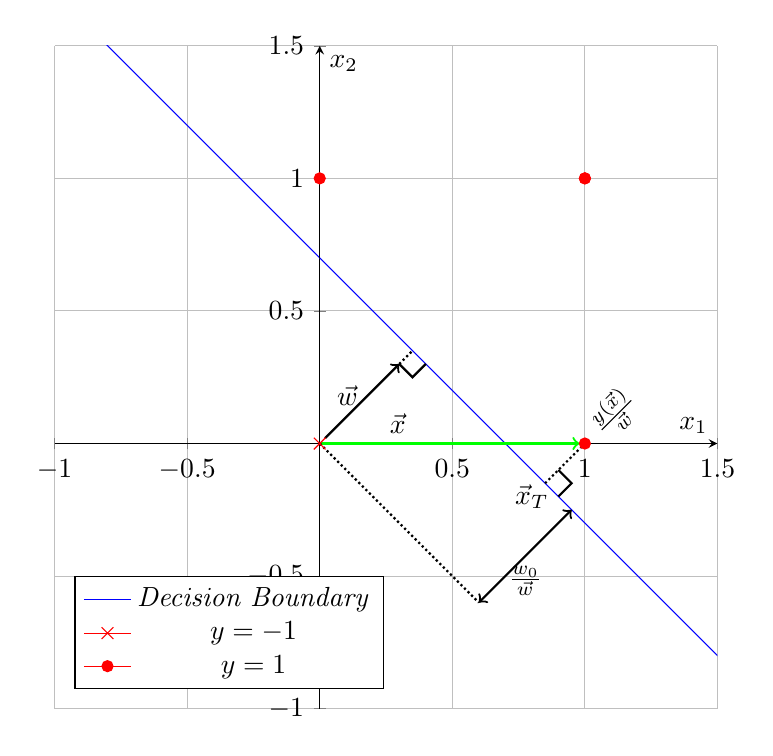
\begin{tikzpicture}
        \begin{axis}[
            xlabel=$x_1$,
            ylabel=$x_2$,
            xmin=-1, xmax=1.5,
            ymin=-1, ymax=1.5,
            grid=major,
            width=10cm,
            height=10cm,
            domain=-2:4,
            samples=100,
            legend pos=south west,
            axis lines=middle, % Add this line to get the axes in the middle
        ]
        \addplot[color=blue]{-x+0.7};
        % Adding x and y axis
        \draw [dashed] (axis cs:0,-6) -- (axis cs:0,6) node [above] {$x=0$};
        \draw [dashed] (axis cs:-2,0) -- (axis cs:4,0) node [right] {$y=0$};

        % Adding points
        \addplot[mark=x, color=red, mark size = 3] coordinates {(0,0)};
        \addplot[mark=*, color=red, mark size = 2] coordinates {(0,1)};
        \legend{\textit{Decision Boundary}, $y = -1$, $y = 1$}
        \addplot[mark=*, color=red, mark size = 2] coordinates {(1,0)};
        \addplot[mark=*, color=red, mark size = 2] coordinates {(1,1)};
        \addplot[mark=*, color=red, mark size = 2] coordinates {(1,1)};

        % Adding vector
        \draw[->, thick] (axis cs:0.02,0.02) -- (axis cs:0.3,0.3) node[pos=0.3, above] {$\vec{w}$};
        \draw[->, thick, color=green] (axis cs:0,0) -- (axis cs:0.98,0) node[pos=0.3, above, color=black] {$\vec{x}$};
        \draw[thick, densely dotted] (axis cs:0.3,0.3) -- (axis cs:0.35,0.35);
        \draw[<->, thick] (axis cs:0.6,-0.6) -- (axis cs:0.95,-0.25) node[midway, below] {$\frac{w_0}{\lvert\vec{w}\rvert}$};
        \draw[densely dotted, thick] (axis cs:0.85,-0.15) -- (axis cs:1,0) node[pos=1, right, rotate=45, xshift =1mm] {$\frac{y(\vec{x})}{\lvert\vec{w}\rvert}$};
        \node at (axis cs:0.8,-0.2) {$\vec{x}_T$};
        \draw[densely dotted, thick] (axis cs:0,0) -- (axis cs:0.6,-0.6);
        \draw[-, thick] (axis cs:0.3,0.3) -- (axis cs:0.35,0.25) -- (axis cs:0.4,0.3);
        \draw[-, thick] (axis cs:0.9,-0.1) -- (axis cs:0.95,-0.15) -- (axis cs:0.9,-0.2);
        \end{axis}
    \end{tikzpicture}
    \caption{Ilustrasi bagaimana fungsi OR dapat dipisahkan menjadi 2 kelas.}
    \label{fig:plot or}
\end{figure}

Dari gambar \ref{fig:plot or} dapat dilihat terdapat garis biru yang memisahkan kedua label. Terlihat vektor $\vec{w}$ tegak lurus dengan \textit{decision boundary}, dan jarak antara \textit{decision boundary} dan titik origin adalah $\frac{w_0}{\lvert\vec{w}\rvert}$. Kemudian untuk mengetahui jarak antara salah satu titik dengan \textit{decision boundary} melalui persamaan \ref{eq: 2.5}.
\begin{equation}
    r = \frac{y(\vec{x})}{\lvert\vec{w}\rvert}
    \label{eq: 2.5}
\end{equation}
Hal ini dapat dibuktikan dengan memisalkan $\vec{x}_T$ sebagai proyeksi dari titik $\vec{x}$ pada \textit{decision boundary}. Sehingga vektor $\vec{x}$ dapat ditulis seperti pada persamaan \ref{eq: 2.6}.
\begin{equation}
    \vec{x} = \vec{x}_T + r \frac{\vec{w}}{\lvert\vec{w}\rvert}
    \label{eq: 2.6}
\end{equation}
Dengan mengkalikan persamaan \ref{eq: 2.6} dengan $\vec{w}^T$ dan menambahkan $w_0$ didapatkan persamaan \ref{eq: 2.7}.
\begin{equation}
    \vec{w}^T \vec{x} + w_0 = \vec{w}^T \vec{x}_T + w_0 + r \frac{\vec{w}^T \vec{w}}{||\vec{w}||}
    \label{eq: 2.7}
\end{equation}
Karena $y(\vec{x}) = \vec{w}^T \vec{x} + w_0$, $\vec{w}^T \vec{x}_T + w_0 = 0$, dan $\frac{\vec{w}^T \vec{w}}{\lvert\vec{w}\rvert} = \lvert\vec{w}\rvert$. Maka didapatkan persamaan \ref{eq: 2.5}. Untuk memudahkan notasi penulisan terkadang diperkenalkan sebuah \textit{dummy 'input'} berupa $x_0=1$ lalu didefinisikan $\hat{w} = (w_0, \vec{w})$ dan $\hat{x} = (x_0, \vec{x})$ agar dapat ditulis persamaan \ref{eq: 2.8}.
\begin{equation}
    y(\vec{x})=\hat{w}^T\hat{x}
    \label{eq: 2.8}
\end{equation}
Terlihat pada Gambar \ref{fig:plot or} \textit{decision boundary} berhasil memisahkan kedua kelas. Untuk mencari \textit{decision boundary} yang tepat dapat melalui beberapa metode seperti \textit{Support vector machine}, eliminasi gauss, dan regresi linier. Sedangkan metode yang serupa dapat diterapkan dengan jaringan syaraf tiruan. 

\subsection{\textit{Perceptron Algorithm}}

\textit{Perceptron algorithm} adalah algoritma pembelajaran \textit{machine learning} pada \textit{artificial neural network} \cite{Kelleher2019-cj}. \textit{Perceptron} menerima beberapa masukan dan menjumlahkannya. Sebelum keluar dari neuron, isyarat yang dijumlahkan tersebut akan diolah terlebih dahulu dengan memasukkannya ke fungsi aktivasi. Untuk lebih jelas Perhatikan Gambar \ref{fig: Perceptron}. 

\begin{figure}[H]
    \centering
    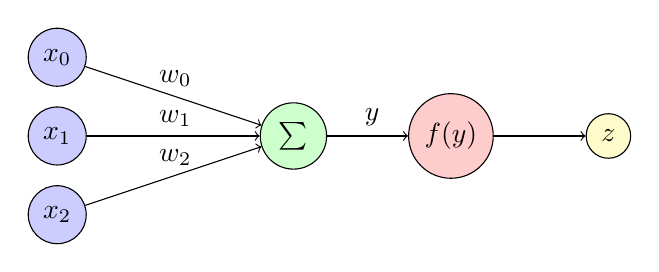
\begin{tikzpicture}

  % Input nodes
  \node[circle, draw, fill=blue!20] (x1) at (0,1) {$x_1$};
  \node[circle, draw, fill=blue!20] (x2) at (0,0) {$x_2$};

  % Weights
  \node[above] at (1.5,1) {$w_1$};
  \node[above] at (1.5,0.5) {$w_2$};

  % Sum node
  \node[circle, draw, fill=green!20] (sum) at (3,1) {$\sum$};
  \node[above] at (4,1) {$y$};

  % Activation node
  \node[circle, draw, fill=red!20] (activation) at (5,1) {$f(y)$};

  % Output node
  \node[circle, draw, fill=yellow!20] (output) at (7,1) {$z$};

  % Bias
  \node[circle, draw, fill=blue!20] (bias) at (0,2) {$x_0$};
  \node[above] at (1.5, 1.5) {$w_0$};

  % Connections
  \draw[->] (x1) -- (sum);
  \draw[->] (x2) -- (sum);
  \draw[->] (bias) -- (sum);
  \draw[->] (sum) -- (activation);
  \draw[->] (activation) -- (output);

\end{tikzpicture}
    \caption{Perceptron yang menerima tiga input dan mengeluarkan satu output}
    \label{fig: Perceptron}
\end{figure}

Gambar \ref{fig: Perceptron} menunjukan unit komputasi terkecil pada \textit{artificial neural network}. Perceptron menerima tiga buah masukan yaitu $x_0$, $x_1$, dan $x_2$. Sedangkan garis-garis penghubung adalah bobot yang masing-masing terhubung dengan tiap-tiap input, bobot-bobot dituliskan dengan simbol $w_0$, $w_1$, dan $w_2$. Kemudian $y$ adalah kombinasi linier antara masukan dan bobotnya seperti pada Persamaan \ref{eq:wx+b}. Setelah melalui kombinasi linier keluaran diolah terlebih dahulu oleh fungsi aktivasi $f(y)$. fungsi aktivasi ini berfungsi untuk menentukan seberapa aktif neuron tersebut. fungsi aktivasi juga memungkinkan jaringan syaraf tiruan dapat mengenali pola masukan dan keluaran yang \textit{non-linear}. Terdapat berbagai macam fungsi aktivasi salah satunya adalah \textit{step function}.

\begin{figure}[H]
    \centering
    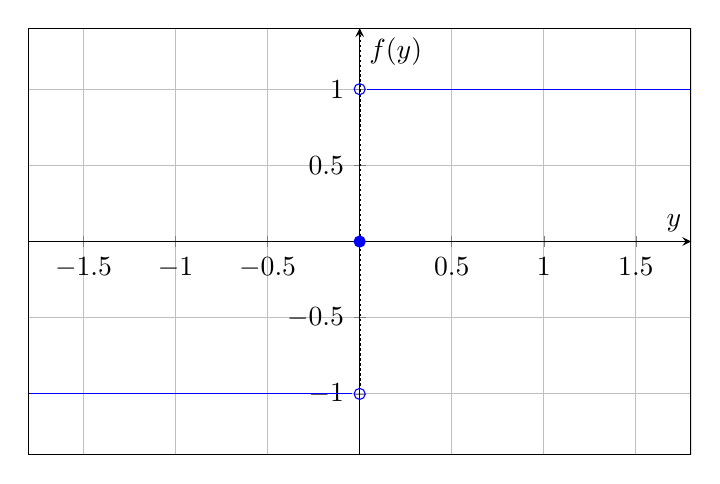
\begin{tikzpicture}
        \begin{axis}[
            xlabel=$y$,
            ylabel=$f(y)$,
            xmin=-1.8, xmax=1.8,
            ymin=-1.4, ymax=1.4,
            width=10cm,
            height=7cm,
            domain=-4:4,
            grid=both,
            samples=100,
            legend pos=south west,
            axis lines=middle, % Add this line to get the axes in the middle
        ]

        % Adding points
        \addplot[mark=*, color=blue, mark size = 2] coordinates {(0,0)};
        \addplot[mark=o, color=blue, mark size = 2] coordinates {(0,1)};
        \addplot[mark=o, color=blue, mark size = 2] coordinates {(0,-1)};

        % Adding line
        \draw[-, color=blue] (axis cs:0.04,1) -- (axis cs:2,1);
        \draw[-, color=blue] (axis cs:-2,-1) -- (axis cs:-0.04,-1);
        \draw[thick, densely dotted] (axis cs:0,96) -- (axis cs:0,-0.96);
        % Draw frame
        \draw[black, thick] (rel axis cs:0,0) rectangle (rel axis cs:1,1);
        \end{axis}
    \end{tikzpicture}
    \caption{Output fungsi aktivasi \textit{step function}}
    \label{fig:plot step_function}
\end{figure}

\textit{Step function} adalah salah satu fungsi aktivasi yang non linier dan tidak kontinu. Keluaran dari \textit{step function} dapat dilihat pada Gambar \ref{fig:plot step_function}. \textit{Step function} dapat ditulis seperti pada Persamaan \ref{eq: Step Function}.
\begin{equation}
    f(y) = 
    \begin{cases} 
    -1 & \text{jika } y < 0 \\
    1 & \text{jika } y \geq 0 
    \end{cases}
    \label{eq: Step Function}
\end{equation}
Pembelajaran \textit{perceptron algorithm} menggunakan \textit{perceptron criterion}. \textit{Perceptron criterion} berupaya menemukan hyperplane yang memisahkan dua kelas titik data. yaitu dengan menggunakan persamaan:
\begin{equation}
    E_p(w)=-\sum_{n \in M}^{}w^T x_n y_n
    \label{eq: perceptron criterion}
\end{equation}
Persamaan \ref{eq: perceptron criterion} berupaya menggunakan \textit{misclassified pattern} untuk melakukan pembelajaran pada \textit{perceptron}, dimana $M$ adalah jumlah \textit{misclassified pattern}. 

\subsection{\textit{Artificial Neural Network}}
Dalam perkembangan \textit{artificial neural network} kerap kali terdapat istilah-istilah yang terdengar serupa tetapi memiliki arti yang berbeda seperti \textit{artificial neural network, machine learning}, dan \textit{deep learning}. Ketiga istilah tersebut memiliki bidang ilmu yang beririsan. \textit{Artificial Neural Network} adalah metode komputasi dari subbidang ilmu \textit{machine learning}, \textit{machine learning} adalah subbidang dari \textit{Artificial Intelligence}, dan \textit{deep learning} merupakan bagian dari \textit{artificial neural network}. Untuk memahami hubungan antara bidang ilmu, dapat dilihat pada Gambar \ref{fig:diagram_venn}.

\begin{figure}[H]
    \centering
    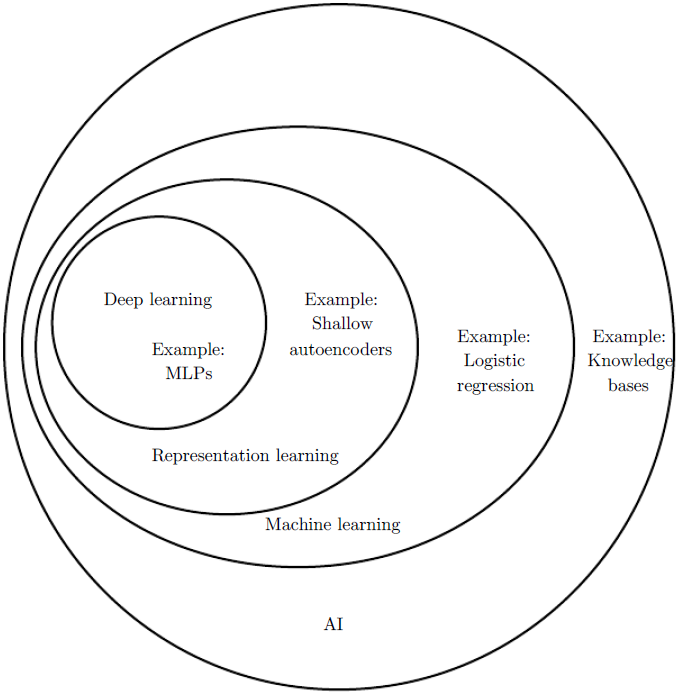
\includegraphics[width = 10cm]{contents/chapter-2/diagram_venn.png}
    \caption{Diagram Venn ini menggambarkan bahwa \textit{deep learning} adalah bagian dari \textit{representation learning}, yang merupakan bagian dari \textit{machine learning}, yang mana digunakan dalam berbagai pendekatan AI, meskipun tidak semuanya. Di dalam setiap bagian diagram, terdapat contohnya.\cite{GoodBengCour16}}
    \label{fig:diagram_venn}
\end{figure}

\textit{Artificial neural networks} terinspirasi dari jaringan syaraf biologis pada otak manusia\cite{Kelleher2019-cj}. Pada otak manusia \textit{neuron-neuron} berkomunikasi satu sama lain melalui sinyal listrik dan ikatan kimia. Sedangkan pada jaringan syaraf tiruan keduanya digantikan dengan model matematika. Sinyal ini diteruskan pada tiap \textit{neuron} dengan sesuatu yang disebut sebagai \textit{action potensial}. Seperti pada Gambar \ref{fig:action potential}. \textit{Neuron-neuron} yang saling terhubung ini memiliki \textit{"strength"}.

\begin{figure}[H]
    \centering
    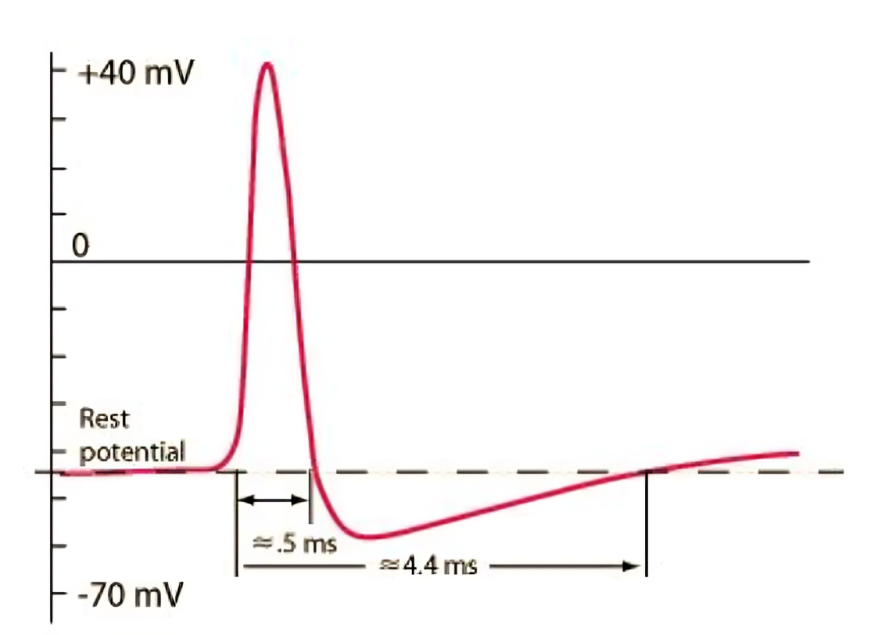
\includegraphics[width=8cm]{contents/chapter-2/action potential.png}
    \caption{\textit{Action Potential} pada jaringan syaraf}
    \label{fig:action potential}
\end{figure}

Jika pada jaringan syaraf manusia setiap \textit{neuron} dapat terhubung dengan \textit{neuron} yang lain, maka pada jaringan syaraf tiruan \textit{neuron-neuron} tersusun teratur membentuk lapisan-lapisan\cite{Kelleher2019-cj}. Tiap-tiap lapisan ini terhubung satu sama lain oleh bobot. Jaringan syaraf tiruan akan menerima sinyal masukan melalui lapisan masukan setelah itu akan diteruskan ke lapisan tersembunyi dan diproses. Langkah selanjutnya tergantung dengan jumlah lapisan tersembunyi, sinyal keluaran dari lapisan tersembunyi dapat diteruskan ke lapisan tersembunyi lainnya atau diteruskan ke lapisan keluaran. Pada lapisan keluaran, sinyal akan diproses dan akan mengeluarkan sinyal keluaran. Kedalaman dari sebuah \textit{neural networks} dapat dilihat dari jumlah lapisan tersembunyi yang dimilikinya. \textit{Neural networks} yang memiliki dua atau lebih lapisan tersembunyi dapat dikatakan sebagai \textit{deep learning}\cite{Kelleher2019-cj}. Arsitektur dari \textit{neural network} digambarkan pada Gambar \ref{fig:2.2 Jaringan Syaraf Tiruan}. 

\begin{figure}[H]
    \centering
    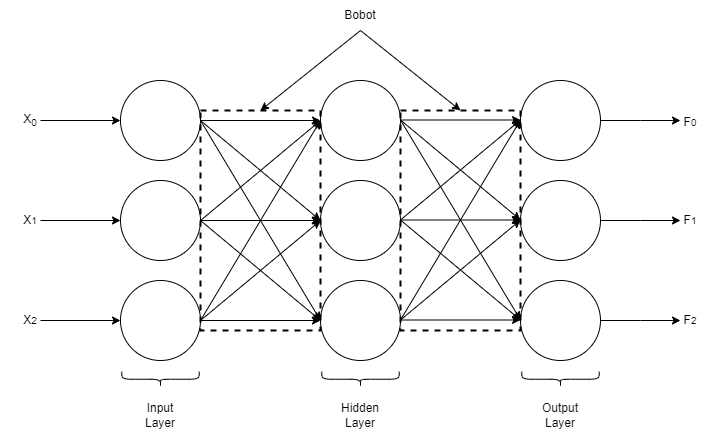
\includegraphics[width = 9cm]{contents/chapter-2/Jaringan Syaraf tiruan.png}
    \caption{Jaringan Syaraf Tiruan}
    \label{fig:2.2 Jaringan Syaraf Tiruan}
\end{figure}

Pada gambar \ref{fig:2.2 Jaringan Syaraf Tiruan} peran dari bobot untuk menunjukkan seberapa kuat hubungan satu \textit{neuron} dengan \textit{neuron} yang lainnya seperti halnya \textit{"strength"} yang ada pada jaringan syaraf. Saat melakukan pelatihan, nilai dari bobot tersebut akan diperbaharui berdasarkan hubungan antara target yang ingin dicapai \textit{expected value} dan sinyal keluarannya \textit{predicted value}. Pelatihan pada \textit{neural network} dapat diartikan sebagai pencarian nilai bobot terbaik\cite{Kelleher2019-cj}. Terdapat berbagai macam arsitektur pada model \textit{artificial neural network}. \textit{multilayer perceptron, reccurent neural networks, convolutional neural networks} dan lainnya. Setiap arsitektur memiliki karakter yang berbeda dan memiliki kecocokan yang berbeda terhadap tipe data tertentu. Contohnya \textit{reccurent neural network} yang baik pada data kontinu seperti isyarat suara sehingga dapat digunakan pada pengenalan suara dan \textit{convolutional neural network} yang baik pada data berbentuk grid sehingga cocok digunakan pada pengenalan gambar.

\subsubsection{Arsitektur \textit{Artificial Neural Network}}

Arsitektur dari jaringan syaraf tiruan mempengaruhi pelatihan dan hasil yang keluar. Pengembangan jaringan syaraf tiruan meliputi pemilihan jenis arsitektur, pemilihan jumlah lapisan tersembunyi ,dan pemilihan jumlah \textit{neuron} pada tiap lapisan \cite{Kelleher2019-cj}. \textit{Neuron} pada lapisan masukan akan mengikuti jumlah \textit{feature} yang diberikan oleh data ditambah 1 untuk merepresentasikan \textit{bias}. \textit{Neuron} pada lapisan keluaran akan mengikuti jumlah kelas K dari data. Sedangkan jenis arsitektur, jumlah \textit{neuron}, dan jumlah lapisan pada lapisan tersembunyi disesuaikan dengan model yang dibutuhkan.

\begin{enumerate}
    \item \textit{Multilayer Perceptron}
    
    Gambar \ref{fig:2.2 Jaringan Syaraf Tiruan} adalah contoh jenis arsitektur \textit{neural network}. Jenis arsitektur ini merupakan yang pertama kali muncul dibanding dengan jenis lainnya. Arsitektur memiliki alur informasi yang bergerak maju atau disebut juga \textit{feedforward neural network} \cite{bishop_2006}. Dapat digunakan untuk jenis data yang berbentuk tabular dan penyelesaian masalah regresi atau klasifikasi sederhana.
    \item \textit{Convolutional Neural Network}

    \begin{figure}[H]
        \centering
        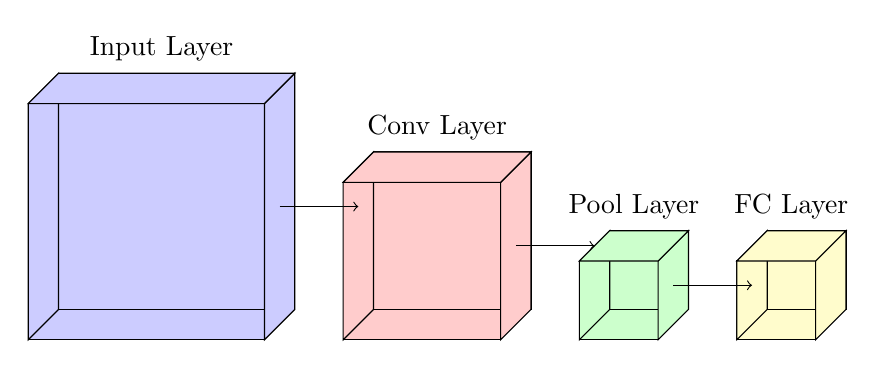
\begin{tikzpicture}

        % Input Layer
        \draw[fill=blue!20] (0,0,0) -- (3,0,0) -- (3,3,0) -- (0,3,0) -- cycle;
        \draw[fill=blue!20] (0,0,-1) -- (3,0,-1) -- (3,3,-1) -- (0,3,-1) -- cycle;
        \draw[fill=blue!20] (0,0,0) -- (0,0,-1) -- (0,3,-1) -- (0,3,0) -- cycle;
        \draw[fill=blue!20] (3,0,0) -- (3,0,-1) -- (3,3,-1) -- (3,3,0) -- cycle;
        \draw[fill=blue!20] (0,3,0) -- (0,3,-1) -- (3,3,-1) -- (3,3,0) -- cycle;

        \node at (1.5, 3.5, -0.5) {Input Layer};

        % Convolutional Layer
        \draw[fill=red!20] (4,0,0) -- (6,0,0) -- (6,2,0) -- (4,2,0) -- cycle;
        \draw[fill=red!20] (4,0,-1) -- (6,0,-1) -- (6,2,-1) -- (4,2,-1) -- cycle;
        \draw[fill=red!20] (4,0,0) -- (4,0,-1) -- (4,2,-1) -- (4,2,0) -- cycle;
        \draw[fill=red!20] (6,0,0) -- (6,0,-1) -- (6,2,-1) -- (6,2,0) -- cycle;
        \draw[fill=red!20] (4,2,0) -- (4,2,-1) -- (6,2,-1) -- (6,2,0) -- cycle;

        \node at (5, 2.5, -0.5) {Conv Layer};

        % Pooling Layer
        \draw[fill=green!20] (7,0,0) -- (8,0,0) -- (8,1,0) -- (7,1,0) -- cycle;
        \draw[fill=green!20] (7,0,-1) -- (8,0,-1) -- (8,1,-1) -- (7,1,-1) -- cycle;
        \draw[fill=green!20] (7,0,0) -- (7,0,-1) -- (7,1,-1) -- (7,1,0) -- cycle;
        \draw[fill=green!20] (8,0,0) -- (8,0,-1) -- (8,1,-1) -- (8,1,0) -- cycle;
        \draw[fill=green!20] (7,1,0) -- (7,1,-1) -- (8,1,-1) -- (8,1,0) -- cycle;
        
        \node at (7.5, 1.5, -0.5) {Pool Layer};
        
        % Fully Connected Layer
        \draw[fill=yellow!20] (9,0,0) -- (10,0,0) -- (10,1,0) -- (9,1,0) -- cycle;
        \draw[fill=yellow!20] (9,0,-1) -- (10,0,-1) -- (10,1,-1) -- (9,1,-1) -- cycle;
        \draw[fill=yellow!20] (9,0,0) -- (9,0,-1) -- (9,1,-1) -- (9,1,0) -- cycle;
        \draw[fill=yellow!20] (10,0,0) -- (10,0,-1) -- (10,1,-1) -- (10,1,0) -- cycle;
        \draw[fill=yellow!20] (9,1,0) -- (9,1,-1) -- (10,1,-1) -- (10,1,0) -- cycle;
        
        \node at (9.5, 1.5, -0.5) {FC Layer};
        
        % Arrows
        \draw[->] (3, 1.5, -0.5) -- (4, 1.5, -0.5);
        \draw[->] (6, 1, -0.5) -- (7, 1, -0.5);
        \draw[->] (8, 0.5, -0.5) -- (9, 0.5, -0.5);
        
        \end{tikzpicture}
        \caption{Arsitektur Convolutional Neural Network}
        \label{fig:Convolutional Neural Network}
    \end{figure}

    Gambar \ref{fig:Convolutional Neural Network} adalah arsitektur \textit{Convolutional Neural Network} (CNN). CNN adalah jenis jaringan syaraf tiruan yang dirancang khusus untuk mengolah data yang memiliki struktur grid, seperti gambar \cite{bishop_2006}. CNN sangat populer dalam tugas-tugas dari bidang \textit{computer vision} seperti pengenalan gambar, deteksi objek, dan segmentasi gambar. CNN terdiri dari beberapa jenis lapisan, masing-masing dengan peran yang spesifik dalam proses pengolahan dan analisis data. Conv Layer berfungsi untuk mengekstrak fitur dari input melalui operasi konvolusi. Pool Layer berfungsi mengurangi dimensi spasial dari fitur untuk mengurangi komputasi dan mencegah overfitting. FC Layer berguna untuk melakukan klasifikasi berdasarkan fitur yang diekstraksi oleh lapisan sebelumnya. CNN juga termasuk kedalam jenis \textit{feedforward neural network}.
    
    \item \textit{Reccurent Neural Network}
    \begin{figure}[H]
        \centering
        \begin{tikzpicture}[->,>=stealth',shorten >=1pt,auto,node distance=3cm,thick,main node/.style={circle,draw,font=\sffamily\Large\bfseries}]

        % Nodes
        \node[main node] (1) {x(t-1)};
        \node[main node] (2) [right of=1] {h(t-1)};
        \node[main node] (3) [right of=2] {h(t)};
        \node[main node] (4) [right of=3] {h(t+1)};
        \node[main node] (5) [above of=2,node distance=2cm] {W};
        \node[main node] (6) [below of=2,node distance=2cm] {U};
        \node[main node] (7) [right of=4] {y(t)};
        
        % Connections
        \path[every node/.style={font=\sffamily\small}]
        (1) edge node [below] {} (2)
            edge node [left] {} (5)
        (2) edge node [left] {} (6)
            edge node [below] {} (3)
        (3) edge node [below] {} (4)
        (4) edge node [below] {} (7)
        (5) edge [bend left] node [left] {} (3)
        (6) edge [bend right] node [left] {} (3);
        
        % Text annotations
        \node at (3.5,1.25) {Hidden State};
        \node at (1.65,-1.3) {Input Weights};
        \node at (5.25,-2.2) {Recurrent Weights};
        
        \end{tikzpicture}
        \caption{Arsitektur \textit{Reccurent Neural Network}}
        \label{fig:Reccurent Neural Network}
    \end{figure}

    Gambar \ref{fig:Reccurent Neural Network} menunjukkan jenis arsitektur \textit{Reccurent Neural Network} (RNN). RNN adalah jenis jaringan syaraf tiruan yang dirancang untuk mengolah informasi data sekuensial \cite{GoodBengCour16}. RNN memiliki kemampuan untuk mengingat informasi dari input sebelumnya dan menggunakan informasi ini untuk mempengaruhi output saat ini. Karena itu RNN sangat berguna untuk tugas-tugas yang melibatkan data sekuensial, seperti \textit{natural language processing} (NLP), pengenalan suara, dan analisis data yang terikat waktu.
    \item \textit{Generative Adversial Network}
    \begin{figure}[H]
        \centering
        \begin{tikzpicture}[->,>=stealth',shorten >=1pt,auto,node distance=1cm,
                    thick,main node/.style={rectangle,draw,font=\sffamily\small\bfseries}]

          % Nodes for Generator
          \node[main node] (z) {Noise $z$};
          \node[main node, below=of z] (G) {Generator $G(z)$};
          \node[main node, below=of G] (G_out) {Fake Data};
        
          % Nodes for Discriminator
          \node[main node, right=of G_out] (D) {Discriminator $D(x)$};
          \node[main node, above=of D] (Real) {Real Data};
          \node[main node, below=of D] (D_out_fake) {Real/Fake};
        
          % Connections for Generator
          \path[every node/.style={font=\sffamily\small}]
            (z) edge (G)
            (G) edge (G_out);
        
          % Connections for Discriminator
          \path[every node/.style={font=\sffamily\small}]
            (Real) edge (D)
            (G_out) edge (D)
            (D) edge (D_out_fake);
        
          % Dashed connection for backpropagation
          \draw[->,dashed] (D_out_fake) -| (G_out);
        
          % Annotations
          \node[align=center] at (1.5,-4.5) {Training Phase};
          
        \end{tikzpicture}
        \caption{Arsitektur \textit{Generative Adversarial Network}}
        \label{fig:arsitektur GAN}
    \end{figure}

    \textit{Generative Adversarial Network} (GAN) adalah sebuah arsitektur jaringan saraf tiruan yang terdiri dari dua model utama: \textit{Generator} dan \textit{Discriminator} \cite{Langr2019-xk}. Ide utama dibalik GAN adalah untuk melatih \textit{Generator} agar dapat menghasilkan data yang sangat mirip dengan data asli yang diberikan, sementara \textit{Discriminator} dilatih untuk membedakan antara data palsu yang dihasilkan oleh \textit{Generator} dan data asli. Jika diskriminator berhasil membedakan data asli dan data yang dibuat oleh generator maka generator dilatih kembali untuk menghasilkan data palsu yang lebih baik. Sedangkan jika diskriminator gagal membedakannya maka diskriminator dilatih kembali hingga dapat membedakan kedua jenis data. Dengan ini kedua model saling berkompetisi untuk menghasilkan model terbaik. GAN biasa digunakan untuk menghasilkan model \textit{Generator} yag serupa dengan data aslinya. Seperti pada \textit{Fake Image Generator}.
\end{enumerate}

\subsection{Normalisasi}
Normalisasi adalah proses mengubah skala data sehingga memiliki karakteristik tertentu yang lebih diinginkan. Nilai suatu data sangat berpengaruh pada pelatihan \textit{neural network}. Algoritma \textit{gradient descent} pada \textit{neural network} bekerja dengan memperbarui bobot berdasarkan \textit{gradien} dari \textit{loss function}. Jika fitur-fitur memiliki skala yang berbeda-beda, \textit{gradien} yang dihitung bisa menjadi sangat besar atau sangat kecil, menyebabkan pembaruan bobot yang tidak seimbang dan mengakibatkan konvergensi yang lambat atau bahkan tidak stabil \cite{Langr2019-xk}. Untuk fitur dengan nilai yang sangat besar, gradien mungkin menjadi sangat besar, menyebabkan langkah-langkah pembaruan bobot yang terlalu besar. Sebaliknya, untuk fitur dengan nilai yang sangat kecil, gradien mungkin menjadi sangat kecil, menyebabkan langkah-langkah pembaruan yang terlalu kecil. Kedua situasi ini dapat membuat algoritma gradient descent tidak efisien atau bahkan gagal konvergen. Sebagai contoh diberikan data seperti pada Tabel \ref{tab:hargarumah}. Misalkan dataset tersebut akan digunakan untuk memprediksi harga rumah.

\begin{table}[H]
    \centering
    \begin{tabular}{||p{5em}|p{5em}|p{5em}|p{5em}|p{6em}||}
    \hline
       Luas Tanah (m²) & Jumlah Kamar Tidur & Usia Rumah (tahun) & Jarak ke Pusat Kota (km) & Harga Rumah (IDR)\\ [0.5ex]
        \hline\hline
       300 & 3 & 10 & 15 & 1,500,000,000\\ \hline
       500 & 4 & 5 & 10 & 2,000,000,000\\ \hline
       450 & 3 & 20 & 20 & 1,750,000,000\\ \hline
       600 & 5 & 8 & 5 &2,500,000,000\\ \hline
    \end{tabular}
    \caption{Data \textit{dummy} harga rumah di Jakarta}
    \label{tab:hargarumah}
\end{table}

Jika data mentah ini langsung digunakan ke algoritma pembelajaran mesin (misalnya, regresi linear), fitur-fitur dengan skala yang lebih besar (seperti luas tanah) akan mendominasi proses pelatihan model. Misalnya, nilai "Luas Tanah" berkisar antara 300 hingga 600, sementara "Jumlah Kamar Tidur" hanya berkisar antara 3 hingga 5. Algoritma mungkin lebih condong ke fitur "Luas Tanah" karena perbedaan skala yang signifikan, meskipun "Jumlah Kamar Tidur" mungkin juga sangat penting dalam menentukan harga rumah.

Untuk mengatasi masalah ini, dapat dilakukan normalisasi pada setiap fitur sehingga semua fitur memiliki skala yang serupa. Salah satu metode normalisasi yang umum adalah Min-Max Scaling, yang mengubah skala setiap fitur ke dalam rentang 0 hingga 1. Persamaan \textit{Min-Max Scaling} (\ref{eq:minmax}):
 \begin{equation}
 x_{norm} = \frac{x-x_{min}}{x-x_{max}}
 \label{eq:minmax}
 \end{equation}
Selain \textit{Min-max scaling}, terdapat metode normalisasi lain  yaitu \textit{Z-score standardization}. \textit{Z-score standardization} adalah metode normalisasi data yang mengubah data sehingga memiliki nilai rata-rata 0 dan standar deviasi 1 \cite{Langr2019-xk}. \textit{Z-score standardization} cenderung lebih tahan terhadap \textit{outlier} dibandingkan dengan \textit{min-max scaling}. Karena z-score didasarkan pada nilai rata-rata dan nilai standar deviasi, \textit{outlier} tidak secara drastis mengubah skala data secara keseluruhan. Persamaan \textit{Z-score standardization} (\ref{eq:Zscore}):
\begin{equation}
    Z=\frac{X-\mu}{\sigma}
    \label{eq:Zscore}
\end{equation}
Dengan $X$ adalah nilai asli data, $\mu$ adalah nilai rata-rata dari data, dan $\sigma$ adalah standar deviasi dari data. Secara garis besar dengan normalisasi, algoritma pembelajaran mesin memberikan bobot yang proporsional kepada setiap fitur berdasarkan informasi yang dikandungnya, bukan berdasarkan skala aslinya. Ini membantu meningkatkan kinerja model dan menghasilkan prediksi yang lebih akurat.

\subsection{\textit{Loss Function}}

\textit{Loss function} adalah parameter yang digunakan untuk mengukur seberapa baik atau buruk kinerja suatu model dalam memprediksi nilai yang benar dari data yang diberikan. \textit{loss function} merupakan komponen penting dalam proses pelatihan model. Dengan menurunkan nilai \textit{loss function} model akan menjadi lebih baik \cite{GoodBengCour16}. Tujuan utama dari \textit{loss function} adalah untuk memberikan umpan balik kepada model terkait seberapa baik model tersebut memperkirakan nilai yang benar dari data yang diamati. Dengan kata lain, \textit{loss function} memberi tahu model seberapa jauh atau dekat prediksi model dengan nilai yang seharusnya.

\subsubsection{\textit{Mean Square Error}}

\textit{Mean Squared Error} (MSE) adalah parameter yang digunakan untuk mengukur rata-rata kuadrat kesalahan antara nilai yang diprediksi oleh model dan nilai sebenarnya \cite{GoodBengCour16}. 
\begin{equation}
    \text{MSE} = \frac{1}{N} \sum_{n=1}^{N} (y_n - \hat{y}_n)^2
    \label{eq:MSE}
\end{equation}
Dimana \(N\) adalah jumlah sampel data, \(y_n\) adalah \textit{expected value} dari sampel ke-n, \(\hat{y}_n\) adalah \textit{predicted value} oleh model untuk sampel ke-n.

\subsubsection{\textit{Binary Cross-Entropy}}

\textit{Binary Cross-Entropy} (BCE) adalah \textit{loss function} yang digunakan dalam permasalan klasifikasi dua kelas atau biner. BCE mengukur perbedaan antara distribusi probabilitas yang diprediksi oleh model dan distribusi probabilitas sebenarnya dari data \cite{bishop_2006}.
\begin{equation}
    L(y, \hat{y}) = - \left( y \log(\hat{y}) + (1 - y) \log(1 - \hat{y}) \right)
\end{equation}
Dimana \(y\) adalah \textit{expected value} (0 atau 1). \(\hat{y}\) adalah probabilitas yang \textit{predicted value} oleh model bahwa label adalah 1 (nilai antara 0 dan 1). Untuk sejumlah \(N\) sampel data, BCE dinyatakan sebagai rata-rata dari semua sampel:
\begin{equation}
    L(Y, \hat{Y}) = - \frac{1}{N} \sum_{n=1}^{N} \left( y_n \log(\hat{y}_n) + (1 - y_n) \log(1 - \hat{y}_n) \right)
\end{equation}

\subsubsection{\textit{Categorical Cross-Entropy Loss}}

\textit{Categorical Cross-Entropy} (CCE) adalah \textit{loss function} yang serupa dengan BCE namun digunakan pada masalah klasifikasi multi-kelas \cite{GoodBengCour16}. CCE mengukur perbedaan antara distribusi probabilitas yang diprediksi oleh model dan distribusi probabilitas sebenarnya dari data.
\begin{equation}
    L(y, \hat{y}) = - \sum_{k=1}^{K} y_k \log(\hat{y}_k)
\end{equation}
Dimana \(K\) adalah jumlah kelas. \(y_k\) adalah \textit{expected value} untuk kelas ke-k (dinyatakan sebagai one-hot encoding). \(\hat{y}_k\) adalah probabilitas \textit{predicted} oleh model untuk kelas ke-k (nilai antara 0 dan 1). Untuk sejumlah \(N\) sampel data, CCE dinyatakan sebagai rata-rata dari semua sampel:
\begin{equation}
    L(Y, \hat{Y}) = - \frac{1}{N} \sum_{n=1}^{N} \sum_{k=1}^{K} y_{nk} \log(\hat{y}_{nk})
\end{equation}

\subsubsection{\textit{Huber Loss}}

\textit{Huber Loss} (HL) adalah \textit{loss function} yang digunakan dalam permasalahan regresi. HL menggabungkan persamaan dari \textit{Mean Squared Error} (MSE) dan \textit{Mean Absolute Error} (MAE) untuk memberikan galat yang lebih \textit{robust} terhadap outliers \cite{Bonaccorso2020-ec}. Untuk satu sampel data, HL didefinisikan sebagai:
\begin{equation}
    L_{\delta}(y, \hat{y}) = 
    \begin{cases} 
    \frac{1}{2}(y - \hat{y})^2 & \text{jika } |y - \hat{y}| \leq \delta \\
    \delta |y - \hat{y}| - \frac{1}{2}\delta^2 & \text{jika } |y - \hat{y}| > \delta
    \end{cases}
\end{equation}
Dimana \(y\) adalah \textit{expected value}. \(\hat{y}\) adalah \textit{predicted value} oleh model. \(\delta\) adalah ambang batas yang menentukan peralihan antara MSE dan MAE. Untuk sejumlah \(N\) sampel data, Huber Loss dinyatakan sebagai rata-rata dari semua sampel:
\begin{equation}
    L_{\delta}(Y, \hat{Y}) = \frac{1}{N} \sum_{n=1}^{N} L_{\delta}(y_n, \hat{y}_n)
\end{equation}

\subsubsection{Kullback-Leibler Divergence (KL Divergence)}

Kullback-Leibler Divergence (KL Divergence) adalah ukuran yang digunakan dalam teori informasi dan statistik untuk mengukur seberapa banyak satu distribusi probabilitas berbeda dari distribusi probabilitas lain \cite{Bonaccorso2020-ec}. Untuk dua distribusi probabilitas \(P\) dan \(Q\), di mana \(P\) adalah distribusi \textit{expected value} dan \(Q\) adalah distribusi dari \textit{predicted value}, KL Divergence dari \(Q\) ke \(P\) didefinisikan sebagai:
\begin{equation}
    D_{KL}(P \parallel Q) = \sum_{x} P(x) \log \left( \frac{P(x)}{Q(x)} \right)
\end{equation}
Jika \(P\) dan \(Q\) adalah distribusi kontinu, maka rumusnya adalah:
\begin{equation}
    D_{KL}(P \parallel Q) = \int_{-\infty}^{\infty} P(x) \log \left( \frac{P(x)}{Q(x)} \right) dx
\end{equation}
KL Divergence tidak simetris, artinya \(D_{KL}(P \parallel Q) \neq D_{KL}(Q \parallel P)\). KL Divergence selalu non-negatif, yaitu \(D_{KL}(P \parallel Q) \geq 0\), dan nol hanya jika \(P = Q\) secara identik. KL Divergence dapat dianggap sebagai jumlah informasi tambahan yang diperlukan untuk mengkodekan distribusi \(P\) menggunakan distribusi \(Q\).

\subsection{\textit{Activasion Function}}

Fungsi aktivasi adalah komponen penting dalam jaringan saraf tiruan yang menentukan keluaran dari suatu \textit{neuron} atau node berdasarkan masukan yang diterima. Fungsi aktivasi memperkenalkan non-linearitas ke dalam model, yang memungkinkan jaringan saraf untuk mempelajari dan memodelkan data yang kompleks, seperti gambar, teks, dan audio. Tanpa fungsi aktivasi, jaringan saraf akan menjadi kombinasi linear dari input, yang membatasi kemampuannya untuk memecahkan masalah non-linear \cite{bishop_2006}. Fungsi \textit{sigmoid} dan \textit{step function} sering digunakan dalam jaringan saraf lapis satu dan pada output untuk tugas klasifikasi biner (0, 1).

\subsubsection{\textit{Step Function}}
\textit{Step function} adalah fungsi yang merubah nilai secara ke 0 dan 1 pada titik-titik tertentu, dan tetap konstan di antara titik-titik tersebut. \textit{Step function} biasanya digunakan dalam permasalahan dimana variabel output hanya dapat mengambil nilai-nilai diskrit tertentu, yang membuatnya berbeda dari fungsi kontinu yang berubah secara halus.

\begin{equation}
    f(x) = \begin{cases} 
0 & \text{jika } x < 0 \\
1 & \text{jika } x \geq 0 
\end{cases}
\end{equation}
Tetapi fungsi ini memiliki kekurangan, Karena $f(x)$ bersifat diskrit. Turunan dari \textit{step function} tidak berguna pada titik mana pun untuk pelatihan. Tepat pada setiap x mendekati 0, turunan tidak terdefinisi dan turunan pada titik lainnya bernilai 0. Oleh karena itu, turunan dari \textit{loss function} yang menggunakan \textit{step function} tidak memberikan informasi tentang bagaimana memperbarui parameter model \cite{GoodBengCour16}.

\subsubsection{\textit{Sigmoid Function}}

Fungsi sigmoid adalah fungsi matematis yang memiliki bentuk kurva berbentuk "S" atau sigmoid. Fungsi ini sering digunakan dalam konteks jaringan saraf tiruan dan statistik untuk mengaktifkan neuron. Fungsi sigmoid mengubah input menjadi nilai antara 0 dan 1 \cite{Kelleher2019-cj}, membuatnya sangat berguna dalam masalah klasifikasi biner. Fungsi sigmoid didefinisikan sebagai:
\begin{equation}
\sigma(x) = \frac{1}{1 + e^{-x}}
\end{equation}
Dimana \( e \) adalah basis dari logaritma natural (sekitar 2.71828), dan \( x \) adalah input fungsi tersebut. Output dari fungsi sigmoid selalu berada di antara 0 dan 1, yaitu \( 0 < \sigma(x) < 1 \). Fungsi sigmoid memperkenalkan non-linearitas ke model, yang memungkinkan jaringan saraf tiruan untuk belajar dan mewakili hubungan yang kompleks dalam data. Saat \( x \) mendekati positif tak terhingga (\( +\infty \)), output dari fungsi sigmoid mendekati 1. Sebaliknya, saat \( x \) mendekati negatif tak terhingga (\( -\infty \)), output mendekati 0. Pada \( x = 0 \), nilai fungsi sigmoid adalah 0.5. Ini berarti input nol memberikan output tengah-tengah antara 0 dan 1. Turunan dari fungsi sigmoid penting dalam algoritma pembelajaran, seperti \textit{backpropagation}. Turunan dari fungsi sigmoid adalah:
\begin{equation}
    \sigma'(x) = \sigma(x) \cdot (1 - \sigma(x))
\end{equation}
Fungsi sigmoid sering digunakan sebagai fungsi aktivasi dalam jaringan saraf tiruan, terutama di lapisan tersembunyi dan keluaran. Dalam permasalahan regresi, fungsi sigmoid digunakan untuk model probabilitas. Fungsi sigmoid memperkenalkan non-linearitas yang penting untuk menangkap hubungan kompleks dalam data. Outputnya berada dalam rentang terbatas [0,1], yang berguna untuk interpretasi sebagai probabilitas. Namun, dalam jaringan \textit{deep learning}, gradien yang dihitung selama \textit{backpropagation} dapat menjadi sangat kecil, menyebabkan pembelajaran menjadi sangat lambat atau bahkan terhenti. Selain itu, output yang selalu positif dapat menyebabkan ketidakseimbangan dalam pembaruan bobot selama pelatihan jaringan saraf tiruan. Fungsi sigmoid adalah komponen penting dalam banyak model pembelajaran mesin, dan pemahamannya sangat penting untuk bekerja dengan jaringan saraf tiruan dan algoritma terkait.

\subsubsection{\textit{Hyperbolic Tangent Function} (tanh)
}

Fungsi tangens hiperbolik, atau \textit{hyperbolic tangent} (tanh), adalah salah satu fungsi aktivasi yang umum digunakan dalam jaringan saraf tiruan. Fungsi ini memetakan nilai input dari seluruh bilangan real ke rentang antara -1 dan 1 \cite{Kelleher2019-cj}.
\begin{equation}
    \tanh(x) = \frac{\sinh(x)}{\cosh(x)} = \frac{e^x - e^{-x}}{e^x + e^{-x}}
\end{equation}
Dimana \(\sinh(x)\) adalah fungsi sinus hiperbolik. \(\cosh(x)\) adalah fungsi kosinus hiperbolik.

\begin{figure}[H]
    \centering
    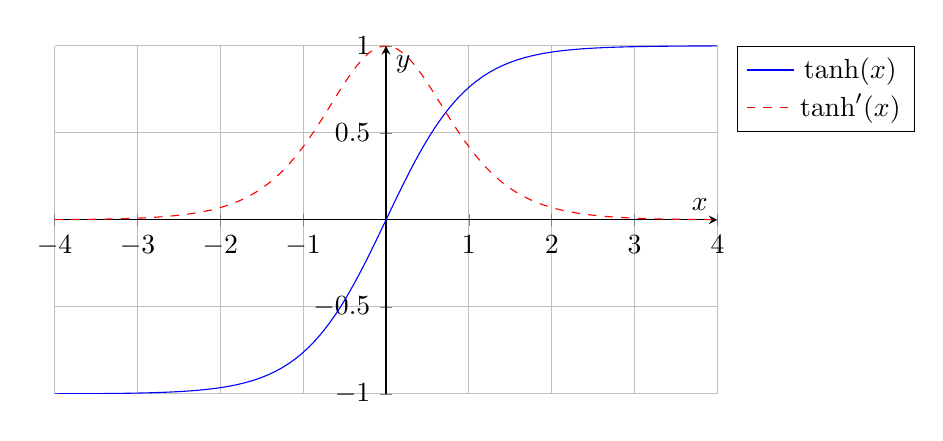
\begin{tikzpicture}
    \begin{axis}[
        domain=-4:4, 
        samples=100, 
        axis lines=center, 
        xlabel=$x$, 
        ylabel=$y$, 
        legend pos=outer north east,
        width=10cm,
        height=6cm,
        grid=major
    ]
    \addplot[color=blue]{tanh(x)};
    \addlegendentry{$\tanh(x)$}
    \addplot[color=red, dashed]{1 - tanh(x)^2};
    \addlegendentry{$\tanh'(x)$}
    \end{axis}
    \end{tikzpicture}
    \caption{\textit{Graph} untuk fungsi tanh(x)}
    \label{fig:tanh}
\end{figure}

Sifat-sifat Fungsi tanh adalah Range \(\tanh(x)\) menghasilkan nilai dalam rentang \([-1, 1]\). Fungsi ini adalah fungsi ganjil, yaitu \(\tanh(-x) = -\tanh(x)\). Turunan dari fungsi tanh adalah:
\begin{equation}
    \tanh'(x) = 1 - \tanh^2(x)
\end{equation}


\subsubsection{\textit{Rectified Linear Unit} (ReLU)}

Fungsi ReLU adalah salah satu fungsi aktivasi yang paling populer dan banyak digunakan dalam jaringan saraf tiruan. Fungsi ReLU mengubah semua nilai negatif menjadi nol dan mempertahankan nilai positif \cite{Kelleher2019-cj}. Fungsi ini populer karena kecepatan konvergensinya yang tinggi dalam \textit{deep learning}. Kelebihan utamanya dalam mengatasi masalah \textit{vanishing gradient} dan membuatnya sangat berguna dalam \textit{deep learning}. ReLU juga membantu dalam konvergensi yang lebih cepat saat pelatihan model, yang sangat penting dalam aplikasi-aplikasi pembelajaran mesin yang membutuhkan waktu pelatihan yang efisien. Fungsi ReLU didefinisikan sebagai:
\begin{equation}
    \text{ReLU}(x) = \max(0, x)
\end{equation}
Rentang keluaran ReLU adalah \([0, \infty)\). Fungsi ini linear ketika \(x\) lebih besar dari atau sama dengan 0. ReLU bisa menghasilkan keluaran nol untuk nilai input negatif. ReLU membantu mengatasi masalah \textit{vanishing gradient}. Fungsi ReLU menghasilkan keluaran nol untuk input negatif, dapat menciptakan banyak kekosongan didalam jaringan. efeknya \textit{neuron-neuron} bisa mati selama pelatihan dan hanya menghasilkan nol. Fungsi ReLU juga tidak memiliki turunan yang terdefinisi dititik nol.

\begin{figure}[H]
    \centering
    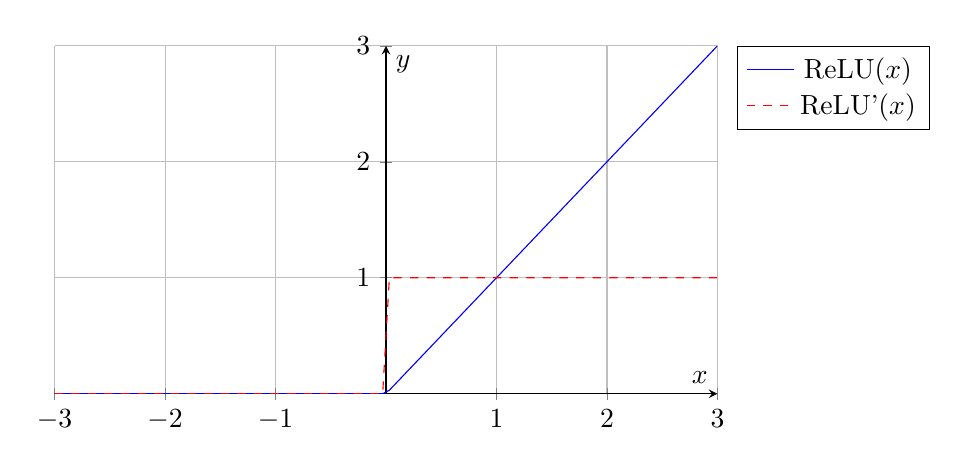
\begin{tikzpicture}
    \begin{axis}[
        domain=-3:3, 
        samples=100, 
        axis lines=center, 
        xlabel=$x$, 
        ylabel=$y$, 
        legend pos=outer north east,
        width=10cm,
        height=6cm,
        grid=major
    ]
    \addplot[color=blue]{max(0,x)};
    \addlegendentry{ReLU($x$)}
    \addplot[color=red, dashed]{x >= 0 ? 1 : 0};
    \addlegendentry{ReLU'($x$)}
    \end{axis}
\end{tikzpicture}
    \caption{\textit{Graph} untuk fungsi ReLU}
    \label{fig:ReLU}
\end{figure}


\subsubsection{\textit{Leaky ReLU}}

Fungsi \textit{Leaky ReLU} adalah variasi dari fungsi aktivasi ReLU yang mengatasi masalah "\textit{dying ReLU}" dimana neuron menjadi tidak aktif dengan memberikan kemiringan kecil untuk nilai negatifnya \cite{Kelleher2019-cj}. Leaky ReLU sering digunakan sebagai fungsi aktivasi dalam lapisan tersembunyi dari jaringan saraf tiruan, terutama ketika ada masalah dengan neuron yang mati selama pelatihan. Dengan menjaga gradien untuk nilai negatif, \textit{Leaky ReLU} membantu memastikan bahwa neuron tetap aktif, sehingga meningkatkan stabilitas dan efisiensi pelatihan model. Leaky ReLU didefinisikan sebagai:
\begin{equation}
    \text{Leaky ReLU}(x) = 
    \begin{cases} 
    x & \text{jika } x \geq 0 \\
    \alpha x & \text{jika } x < 0 
    \end{cases}
\end{equation}
Dimana \(\alpha\) adalah parameter kecil yang menentukan kemiringan untuk nilai negatif. Biasanya, \(\alpha\) diatur ke nilai kecil seperti 0.01. Dengan memberikan gradien kecil untuk nilai negatif, Leaky ReLU membantu menjaga neuron tetap aktif selama pelatihan. Seperti ReLU, fungsi Leaky ReLU juga sederhana untuk dihitung dan sangat efisien dari segi komputasi. Namun pemilihan nilai \(\alpha\) bisa menjadi tantangan tersendiri.
\begin{figure}[H]
    \centering
    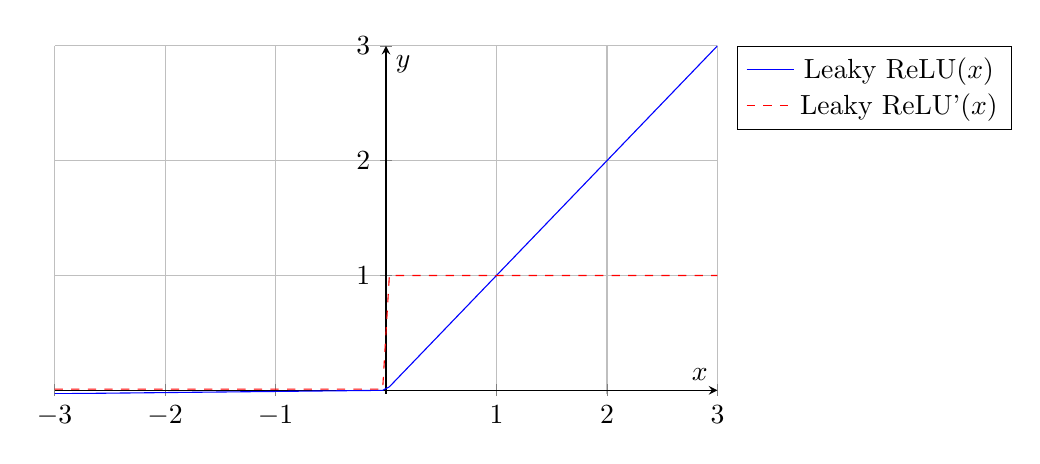
\begin{tikzpicture}
        \begin{axis}[
            domain=-3:3, 
            samples=100, 
            axis lines=center, 
            xlabel=$x$, 
            ylabel=$y$, 
            legend pos=outer north east,
            width=10cm,
            height=6cm,
            grid=major
        ]
        \addplot[color=blue]{x >= 0 ? x : 0.01*x};
        \addlegendentry{Leaky ReLU($x$)}
        \addplot[color=red, dashed]{x >= 0 ? 1 : 0.01};
        \addlegendentry{Leaky ReLU'($x$)}
        \end{axis}
    \end{tikzpicture}
    \caption{\textit{Graph} untuk Leaky ReLU}
    \label{fig:enter-label}
\end{figure}

Rentang keluaran \textit{Leaky ReLU} adalah \((-\infty, \infty)\). Fungsi ini linear untuk \(x \geq 0\) dan memiliki kemiringan kecil (yang ditentukan oleh \(\alpha\)) untuk \(x < 0\). Fungsi \textit{Leaky ReLU} memiliki gradien yang tidak nol untuk nilai negatif.

\subsubsection{\textit{Parametric ReLU} (PReLU)}

Fungsi PReLU adalah variasi dari fungsi aktivasi ReLU yang memperkenalkan parameter $\alpha$ yang dapat dipelajari untuk nilai negatif \cite{GoodBengCour16}. Fungsi PReLU sering digunakan dalam \textit{deep learning}, terutama ketika ada kebutuhan untuk meningkatkan fleksibilitas dan kinerja fungsi aktivasi. Dengan parameter yang dapat dipelajari, PReLU memberikan kemampuan pada model untuk menyesuaikan model lebih baik terhadap data, yang bisa menghasilkan kinerja yang lebih baik dalam berbagai tugas pembelajaran mesin. Fungsi PReLU didefinisikan sebagai:
\begin{equation}
    \text{PReLU}(x) = \begin{cases} 
x & \text{jika } x \geq 0 \\
\alpha x & \text{jika } x < 0 
\end{cases}
\end{equation}
Dimana \(\alpha\) adalah parameter yang dapat dipelajari. Dengan \(\alpha\) sebagai parameter yang dapat dipelajari, fungsi PReLU dapat menyesuaikan dengan data selama pelatihan. PReLU membantu menjaga neuron tetap aktif dengan memiliki gradien yang tidak nol untuk nilai negatif. Nilai \(\alpha\) dioptimalkan selama pelatihan, sehingga model dapat menyesuaikan fungsi aktivasi untuk kinerja terbaik. Namun memperkenalkan parameter yang dapat dipelajari akan menambah kompleksitas pelatihan. Potensi risiko \textit{overfitting} dengan menambahkan lebih banyak parameter yang dapat dipelajari.

\begin{figure}[H]
    \centering
    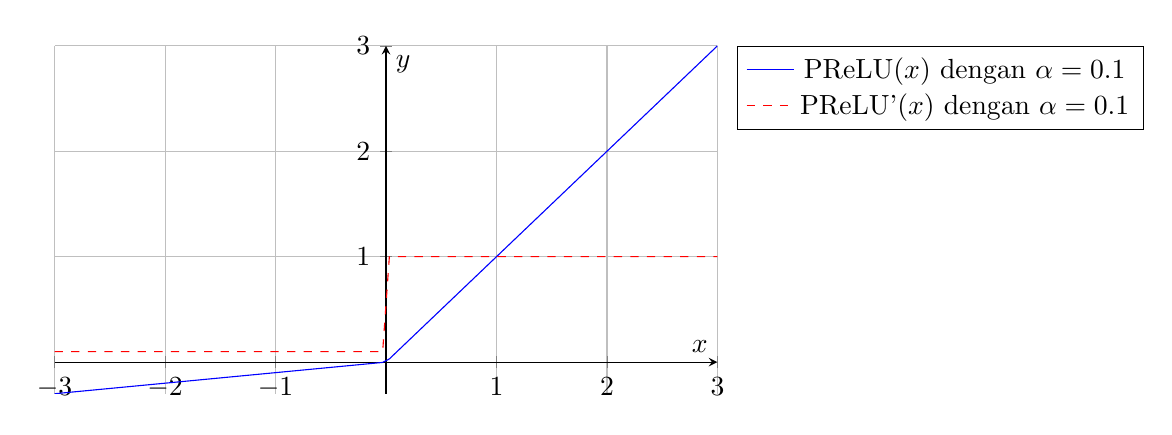
\begin{tikzpicture}
    \begin{axis}[
        domain=-3:3, 
        samples=100, 
        axis lines=center, 
        xlabel=$x$, 
        ylabel=$y$, 
        legend pos=outer north east,
        width=10cm,
        height=6cm,
        grid=major
    ]
    \addplot[color=blue]{x >= 0 ? x : 0.1*x};
    \addlegendentry{PReLU($x$) dengan $\alpha = 0.1$}
    \addplot[color=red, dashed]{x >= 0 ? 1 : 0.1};
    \addlegendentry{PReLU'($x$) dengan $\alpha = 0.1$}
    \end{axis}
    \end{tikzpicture}
    \caption{\textit{Graph} untuk Parametric ReLU}
    \label{fig:enter-label}
\end{figure}

Rentang keluaran PReLU adalah \((-\infty, \infty)\). Fungsi ini linear untuk \(x \geq 0\) dan linear dengan kemiringan \(\alpha\) untuk \(x < 0\). Fungsi PReLU memiliki gradien yang tidak nol untuk nilai negatif.

\subsubsection{\textit{Exponential Linear Unit} (ELU)}

Fungsi ELU adalah fungsi aktivasi yang memberikan nilai negatif untuk input negatif dan memiliki turunan yang lebih halus, yang membantu dalam mempercepat pelatihan dan mengatasi masalah "\textit{dying ReLU}". Fungsi ELU juga cukup sering digunakan dalam \textit{deep learning}, terutama ketika ada kebutuhan untuk mengatasi masalah "\textit{dying ReLU}" dan mempercepat konvergensi \cite{Bonaccorso2020-ec}. Dengan memiliki saturasi negatif dan gradien halus, ELU dapat membantu model untuk belajar lebih efisien dan mencapai kinerja yang lebih baik dalam berbagai tugas pembelajaran mesin. Fungsi ELU didefinisikan sebagai:
\begin{equation}
    \text{ELU}(x) = \begin{cases} 
x & \text{jika } x \geq 0 \\
\alpha (e^x - 1) & \text{jika } x < 0 
\end{cases}
\end{equation}
Dimana \(\alpha\) adalah parameter positif yang menentukan kemiringan untuk nilai negatif. ELU memberikan nilai negatif untuk input negatif, membantu menjaga neuron tetap aktif. ELU memiliki saturasi negatif yang membantu mempercepat konvergensi. Turunan dari ELU lebih halus dibandingkan dengan ReLU. Menghitung eksponensial untuk nilai negatif bisa lebih mahal secara komputasi. Pemilihan nilai \(\alpha\) bisa mempengaruhi performa model.

\begin{figure}[H]
    \centering
    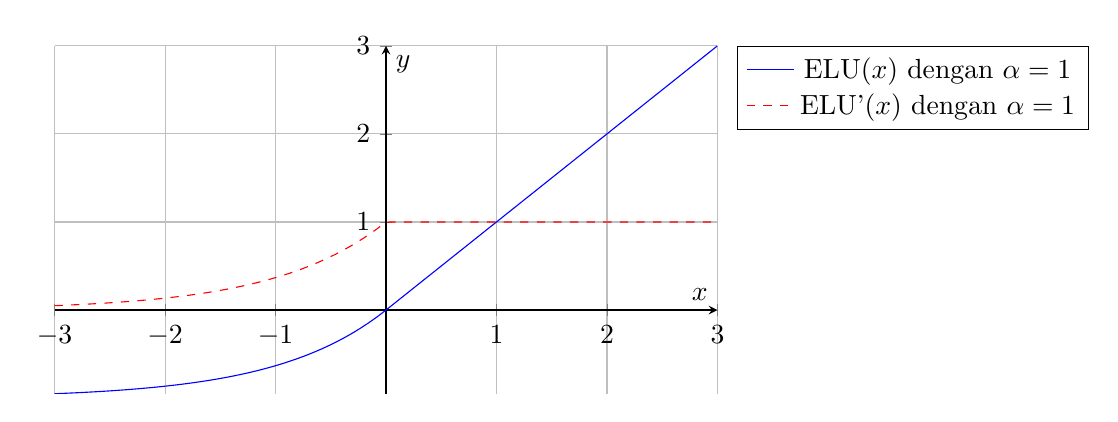
\begin{tikzpicture}
    \begin{axis}[
        domain=-3:3, 
        samples=100, 
        axis lines=center, 
        xlabel=$x$, 
        ylabel=$y$, 
        legend pos=outer north east,
        width=10cm,
        height=6cm,
        grid=major
    ]
    \addplot[color=blue]{x >= 0 ? x : 1*(exp(x)-1)};
    \addlegendentry{ELU($x$) dengan $\alpha = 1$}
    \addplot[color=red, dashed]{x >= 0 ? 1 : exp(x)};
    \addlegendentry{ELU'($x$) dengan $\alpha = 1$}
    \end{axis}
    \end{tikzpicture}
    \caption{\textit{Graph} untuk ELU}
    \label{fig:enter-label}
\end{figure}

Rentang keluaran ELU adalah \([-\alpha, \infty)\). ELU memiliki saturasi negatif untuk nilai \(x\) negatif yang besar. Fungsi ini linear untuk \(x \geq 0\).

\subsubsection{Softmax}

Fungsi ini mengubah nilai menjadi distribusi probabilitas \cite{bishop_2006}. Fungsi ini biasanya digunakan di lapisan output untuk tugas klasifikasi.
\begin{figure}[H]
    \centering
    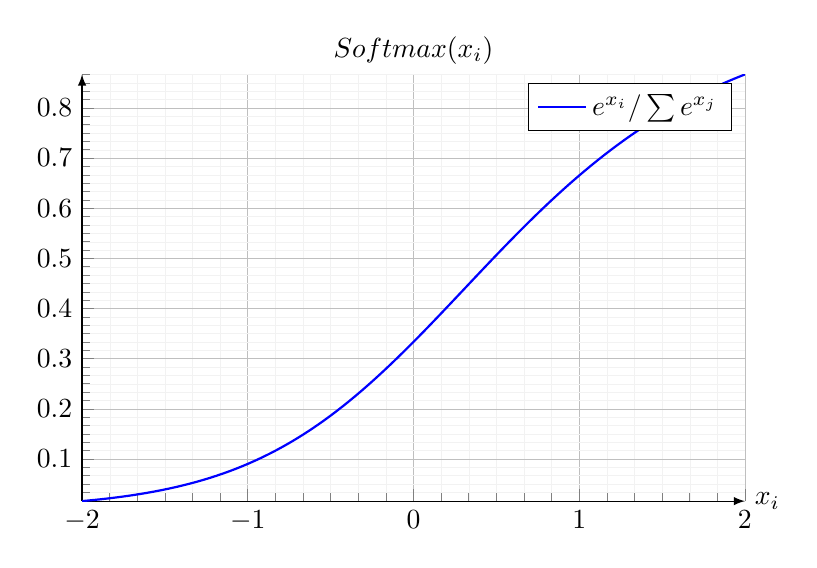
\begin{tikzpicture}
    \begin{axis}[
        xlabel={$x_i$},
        ylabel={$\text{Softmax}(x_i)$},
        grid=both,
        grid style={line width=.1pt, draw=gray!10},
        major grid style={line width=.2pt,draw=gray!50},
        minor tick num=5,
        width=10cm,
        height=7cm,
        domain=-2:2,
        samples=100,
        xtick={-2,-1,...,2},
        ytick={0,0.1,...,1},
        enlargelimits=false,
        axis lines*=left,
        every axis y label/.style={at={(current axis.above origin)},anchor=south},
        every axis x label/.style={at={(current axis.right of origin)},anchor=west},
        axis line style={-latex}
    ]
    \addplot[thick,blue] {exp(x)/(exp(x) + exp(0) + exp(-x))};
    \addlegendentry{$e^{x_i}/\sum e^{x_j}$}
    \end{axis}
\end{tikzpicture}
    \caption{\textit{Graph} untuk fungsi softmax}
    \label{fig:enter-label}
\end{figure}
Fungsi ini memastikan bahwa output jaringan adalah distribusi probabilitas, yang sangat berguna untuk menentukan kelas yang paling mungkin dari sebuah input. Softmax juga memungkinkan penggunaan \textit{loss function} seperti \textit{categorical cross-entropy}, yang menghitung kesalahan antara distribusi prediksi dan distribusi target. Fungsi softmax untuk elemen \( i \) dari vektor input \( \mathbf{z} \) didefinisikan sebagai:
\begin{equation}
    \text{softmax}(z_i) = \frac{e^{z_i}}{\sum_{j=1}^{K} e^{z_j}}
\end{equation}

\subsection{Gradient Descent}

Gradient descent adalah algoritma optimasi yang digunakan untuk meminimalkan \textit{loss function} dalam berbagai model pembelajaran mesin dan jaringan saraf tiruan. Inti dari algoritma ini adalah memperbarui parameter model secara iteratif untuk mengurangi nilai \textit{loss function} \cite{bishop_2006}. Proses ini dilakukan dengan mengikuti arah gradien dari \textit{loss function}.
\begin{equation}
    \theta_{t+1} = \theta_t - \eta \nabla_\theta J(\theta_t)
    \label{eq:pembaharuan bobot}
\end{equation}
Dimana $(\theta_t)$ adalah parameter pada iterasi ke-\(t\). \(\eta\) adalah laju pembelajaran (\textit{learning rate}). \(\nabla_\theta J(\theta_t)\) adalah gradien dari \textit{loss function} \(J\) terhadap parameter \(\theta\) pada iterasi ke-\(t\). Cara kerja gradient descent dimulai dengan inisialisasi parameter model $(\theta)$ secara acak atau dengan nilai tertentu. Setelah itu, \textit{loss function} $J(\theta)$ dievaluasi berdasarkan parameter saat ini dan data pelatihan. Langkah selanjutnya adalah menghitung gradien dari \textit{loss function} terhadap parameter. Gradien adalah vektor yang menunjukkan arah dan laju perubahan terbesar dari \textit{loss function}, yang secara matematis dinyatakan sebagai $\nabla_\theta J(\theta)$. Parameter kemudian diperbarui dengan bergerak ke arah gradien negatif untuk mengurangi nilai \textit{loss function}. Pembaruan parameter dilakukan dengan menggunakan persamaan \ref{eq:pembaharuan bobot}, dimana $\eta$ adalah learning rate yang menentukan ukuran langkah yang diambil menuju minimum \textit{loss function}. Langkah-langkah ini diulangi sampai \textit{loss function} konvergen ke nilai minimum atau perubahan dalam \textit{loss function} menjadi sangat kecil.

\subsubsection{Varian Gradient Descent}
Gradient descent adalah algoritma inti dalam optimasi model pembelajaran mesin. Dengan memilih varian yang sesuai dan menggunakan teknik optimasi, model dapat dilatih dengan lebih efisien dan efektif, mencapai konvergensi yang lebih cepat dan hasil yang lebih baik.

\begin{enumerate}
    \item Batch Gradient Descent: Menggunakan seluruh dataset untuk menghitung gradien dan memperbarui parameter \cite{GoodBengCour16}. Kelebihannya adalah konvergen menuju minimum global dengan lebih stabil, namun memerlukan komputasi yang besar jika dataset sangat besar.
    
    \item Stochastic Gradient Descent (SGD): Menggunakan satu contoh data untuk menghitung gradien dan memperbarui parameter \cite{GoodBengCour16}. Kelebihannya adalah lebih cepat dan lebih efisien untuk dataset besar, namun gradien yang dihitung lebih bising sehingga jalur konvergensi bisa lebih berliku-liku.

    \item Mini-Batch Gradient Descent: Kombinasi antara batch gradient descent dan SGD. Menggunakan batch kecil (mini-batch) dari dataset untuk menghitung gradien dan memperbarui parameter \cite{GoodBengCour16}. Pendekatan ini menggabungkan kecepatan dan efisiensi dari SGD dengan kestabilan batch gradient descent.
\end{enumerate}

\subsubsection{Optimasi Gradient Descent}
Untuk meningkatkan kinerja dan konvergensi gradient descent, beberapa teknik dan varian optimasi dapat digunakan:

\begin{enumerate}
    \item \textit{Momentum}
    
    Momentum adalah teknik yang digunakan dalam algoritma optimasi gradient descent untuk mempercepat konvergensi dan mengatasi masalah terjebak pada lokal minima. Prinsip dasar momentum adalah memperhitungkan gradien sebelumnya untuk menentukan arah dan jarak perpindahan parameter dalam proses optimasi \cite{GoodBengCour16}. Dengan momentum, pembaruan parameter dilakukan sebagai berikut:
    \begin{equation}
        v_t = \beta v_{t-1} + (1 - \beta) \nabla_\theta J(\theta_t)
    \end{equation}
    \begin{equation}
        \theta_{t+1} = \theta_t - \eta v_t
    \end{equation}
    Dimana \(v_t\) adalah variabel momentum pada iterasi ke-\(t\). Koefisien momentum \(\beta\) biasanya dipilih antara 0.5 dan 0.9. Bagian dari gradien sebelumnya yang dibawa ke iterasi berikutnya ditunjukkan oleh \(v_{t-1}\). Semakin besar nilai \(\beta\), semakin besar pengaruh gradien sebelumnya terhadap perbaruan parameter. Gradien dari iterasi saat ini diberikan oleh \((1 - \beta) \nabla_\theta J(\theta_t)\). Dengan menggunakan momentum, pembaruan parameter menjadi lebih stabil dan cepat. Gradien sebelumnya membantu memperlancar jalur perpindahan parameter, yang memungkinkan algoritma optimasi mencapai konvergensi dengan lebih efisien.
    
    \item \textit{AdaGrad}
    
    Adagrad digunakan untuk merubah nilai \textit{learning rate} menyesuaikan dengan gradien yang didapat. Adagrad sangat berguna dalam situasi dimana fitur jarang muncul atau terdapat perbedaan skala yang signifikan antara fitur-fitur dalam dataset. Algoritma ini secara otomatis menyesuaikan \textit{learning rate} berdasarkan frekuensi pembaharuan parameter, sehingga fitur yang jarang muncul mendapatkan pembaruan yang lebih besar. Adagrad mengurangi kebutuhan untuk melakukan pencarian \textit{learning rate} yang optimal \cite{GoodBengCour16}. Seiring waktu, laju pembelajaran bisa menjadi sangat kecil karena penjumlahan kuadrat gradien yang terus bertambah, sehingga pembaruan parameter menjadi sangat lambat. Adagrad kurang efektif jika terdapat perubahan skala yang sangat besar antara fitur. Dalam algoritma Adagrad, parameter diperbarui dengan cara sebagai berikut:
    \begin{equation}
        \theta_{t+1} = \theta_t - \frac{\eta}{\sqrt{G_{t, ii} + \epsilon}} \cdot \nabla_{\theta_t} J(\theta_t)
    \end{equation}
    \begin{equation}
        G_{t, ii} = G_{t-1, ii} + (\nabla_{\theta_t} J(\theta_t))^2
        \label{eq:G}
    \end{equation}
    Dimana \(\theta_t\) adalah parameter pada iterasi ke-\(t\). \(\eta\) adalah laju pembelajaran awal (learning rate). \(\nabla_{\theta_t} J(\theta_t)\) adalah gradien dari fungsi biaya \(J\) terhadap parameter \(\theta\) pada iterasi ke-\(t\). \(G_t\) adalah matriks diagonal yang menyimpan jumlah kuadrat dari gradien untuk setiap parameter hingga iterasi ke-\(t\). \(\epsilon\) adalah nilai kecil (biasanya \(10^{-8}\)) untuk mencegah pembagian dengan nol. Sedangkan \(G_{t, ii}\) diperbarui dengan Persamaan \ref{eq:G}. Dimana \(G_{t, ii}\) menyimpan jumlah kuadrat gradien dari iterasi sebelumnya hingga iterasi ke-\(t\) untuk parameter \(\theta_t\).
    
    \item \textit{RMSProp}
    
    RMSprop ini adalah perbaikan dari Adagrad dan dirancang untuk mengatasi beberapa kelemahan dari Adagrad, khususnya masalah peluruhan laju pembelajaran yang terlalu cepat \cite{GoodBengCour16}. RMSprop memperbaiki Adagrad dengan memperkenalkan faktor peluruhan eksponensial untuk menyimpan rata-rata kuadrat gradien sebelumnya. Dengan cara ini, RMSprop menjaga \textit{learning rate} tetap besar dan stabil sepanjang proses pelatihan. Dalam RMSprop, parameter diperbarui dengan cara sebagai berikut:
    \begin{equation}
        \theta_{t+1} = \theta_t - \frac{\eta}{\sqrt{E[g^2]_t + \epsilon}} \cdot \nabla_{\theta_t} J(\theta_t)
    \end{equation}
    \begin{equation}
        E[g^2]_t = \gamma E[g^2]_{t-1} + (1 - \gamma) (\nabla_{\theta_t} J(\theta_t))^2
    \end{equation}
    Dimana \(\theta_t\) adalah parameter pada iterasi ke-\(t\). \(\eta\) adalah laju pembelajaran (learning rate). \(\nabla_{\theta_t} J(\theta_t)\) adalah gradien dari fungsi biaya \(J\) terhadap parameter \(\theta\) pada iterasi ke-\(t\). \(E[g^2]_t\) adalah rata-rata eksponensial dari kuadrat gradien. \(\epsilon\) adalah nilai kecil (biasanya \(10^{-8}\)) untuk mencegah pembagian dengan nol. \(\gamma\) adalah faktor peluruhan, biasanya dipilih antara 0.9 dan 0.99. \(E[g^2]_t\) menyimpan rata-rata eksponensial dari kuadrat gradien pada iterasi ke-\(t\). Dengan menggunakan rata-rata eksponensial dari kuadrat gradien, RMSprop menjaga laju pembelajaran tetap besar dan stabil sepanjang proses pelatihan. RMSprop menyesuaikan \textit{learning rate} untuk setiap parameter, sehingga efektif dalam menangani fitur yang jarang muncul dan data dengan skala yang berbeda. Memilih nilai yang tepat untuk \(\gamma\) dan \(\eta\) bisa memerlukan beberapa eksperimen. Menyimpan dan memperbarui rata-rata eksponensial dari kuadrat gradien juga menambah beban komputasi.
    
    \item \textit{Adam (Adaptive Moment Estimation)}
    
    Adam adalah algoritma optimasi yang populer digunakan dalam pelatihan jaringan syaraf tiruan. Algoritma ini menggabungkan keuntungan dari dua algoritma optimasi lainnya, yaitu RMSprop dan Momentum. Adam secara dinamis menyesuaikan \textit{learning rate} untuk setiap parameter berdasarkan estimasi momen pertama (rata-rata eksponensial dari gradien) dan momen kedua (rata-rata eksponensial dari kuadrat gradien) \cite{GoodBengCour16}. Adam menggunakan dua perkiraan momen, yaitu momen pertama (mean) dan momen kedua (variance), untuk mengendalikan pembaruan parameter. Dengan ini, Adam dapat mengatasi masalah peluruhan \textit{learning rate} yang cepat dan juga menangani gradien yang jarang muncul dengan lebih efektif. Pembaharuan parameter dengan menggunakan persamaan \ref{eq: adam}
    \begin{equation}
        \theta_{t+1} = \theta_t - \frac{\eta}{\sqrt{\hat{v}_t} + \epsilon} \hat{m}_t
        \label{eq: adam}
    \end{equation}
    Dimana \(\theta_t\) adalah parameter yang dilatih pada iterasi ke-\(t\). \(\eta\) adalah \textit{learning rate}. \(\hat{m}_t\) adalah momen pertama. \(\hat{v}_t\) adalah momen kedua. \(\epsilon\) adalah nilai kecil (biasanya \(10^{-8}\)) untuk mencegah pembagian dengan nol. Momen pertama dan kedua diperbaharui dengan persamaan \ref{eq: mhat} dan \ref{eq: vhat}.
    \begin{equation}
        m_t = \beta_1 m_{t-1} + (1 - \beta_1) \nabla_{\theta_t} J(\theta_t)
    \end{equation}
    \begin{equation}
        v_t = \beta_2 v_{t-1} + (1 - \beta_2) (\nabla_{\theta_t} J(\theta_t))^2
    \end{equation}
    \begin{equation}
        \hat{m}_t = \frac{m_t}{1 - \beta_1^t}
        \label{eq: mhat}
    \end{equation}
    \begin{equation}
        \hat{v}_t = \frac{v_t}{1 - \beta_2^t}
        \label{eq: vhat}
    \end{equation}
    Dimana \(\nabla_{\theta_t} J(\theta_t)\) adalah gradien dari fungsi biaya \(J\) terhadap parameter \(\theta\) pada iterasi ke-\(t\). \(m_t\) adalah momen pertama (rata-rata eksponensial dari gradien). \(v_t\) adalah momen kedua (rata-rata eksponensial dari kuadrat gradien). \(\beta_1\) dan \(\beta_2\) adalah faktor peluruhan untuk momen pertama dan kedua, biasanya dipilih sebagai \(\beta_1 = 0.9\) dan \(\beta_2 = 0.999\). Dengan menggabungkan RMSprop dan Momentum, Adam sering kali mencapai konvergensi lebih cepat dan lebih stabil dibandingkan dengan algoritma optimasi lainnya. Adam biasanya memerlukan sedikit penyetelan hyperparameter, membuatnya lebih mudah digunakan dalam berbagai masalah optimasi. Namun menyimpan momen pertama dan kedua membutuhkan lebih banyak memori dibandingkan dengan algoritma seperti Stochastic Gradient Descent (SGD). Meskipun Adam biasanya bekerja dengan baik tanpa banyak penyetelan, dalam beberapa kasus tertentu, pemilihan hyperparameter bisa mempengaruhi kinerjanya secara signifikan.
    
    
\end{enumerate}

\subsection{\textit{Backpropagation}}

\textit{Backpropagation} adalah algoritma yang digunakan untuk melatih jaringan saraf tiruan, terutama \textit{deep learning}. Algoritma ini merupakan bagian penting dari proses pembelajaran yang memungkinkan jaringan untuk mengoptimalkan bobot dan biasnya sehingga dapat meminimalkan \textit{loss function} \cite{bishop_2006}. \textit{Backpropagation} adalah singkatan dari \textit{backward propagation of errors}. Algoritma ini bekerja dengan menghitung gradien dari \textit{loss function} terhadap setiap bobot dalam jaringan, kemudian menggunakan gradien ini untuk memperbarui bobot-bobot tersebut.

Proses \textit{backpropagation} terdiri dari dua fase utama: \textit{forward pass} dan \textit{backward pass}. Pada fase \textit{forward pass}, input data dijalankan melalui jaringan untuk menghasilkan \textit{predicted value}. Kemudian, pada fase \textit{backward pass}, kesalahan antara \textit{predicted value} dan \textit{expected value} dihitung dengan \textit{loss function}, dan gradien dari \textit{loss function} terhadap bobot-bobot dihitung untuk memperbarui bobot-bobot tersebut.

Langkah-langkah dalam \textit{backpropagation} dimulai dengan inisialisasi bobot dan bias secara acak atau dengan nilai tertentu. Pada \textit{forward pass}, input data diberikan ke lapisan input jaringan. Setiap neuron dalam lapisan tersembunyi dan lapisan output menghitung nilai aktivasinya berdasarkan input yang diterima dan fungsi aktivasi yang digunakan. Output dari lapisan terakhir dihitung dan digunakan untuk menghitung \textit{loss function}. Setelah itu, \textit{loss function} \( L(y, \hat{y}) \) dihitung berdasarkan perbedaan antara \textit{expected value} (\( y \)) dan \textit{predicted value} (\( \hat{y} \)). Pada backward pass, gradien dari \textit{loss function} terhadap output dari lapisan terakhir dihitung. Kesalahan ini kemudian dipropagasi mundur melalui jaringan, lapisan demi lapisan, dengan menggunakan aturan rantai (chain rule) untuk menghitung gradien dari \textit{loss function} terhadap setiap bobot. Bobot diperbarui dengan menggunakan gradien yang dihitung selama backward pass. Formula pembaruan bobot adalah:
\[
w_{ij} := w_{ij} - \eta \frac{\partial L}{\partial w_{ij}}
\]
Dimana \( w_{ij} \) adalah bobot antara neuron \( i \) dan neuron \( j \), \( \eta \) adalah learning rate, dan \( \frac{\partial L}{\partial w_{ij}} \) adalah gradien dari \textit{loss function} terhadap bobot tersebut. Langkah-langkah ini diulangi untuk setiap batch data selama beberapa epoch sampai memenuhi kriteria tertentu. Kriteria tersebut dapat berupa \textit{loss function} konvergen ke nilai minimum, \textit{predicted value} sudah serupa dengan \textit{expected value}, iterasi mencapai jumlah yang ditentukan, atau dengan menggunakan \textit{relative error}.

\subsection{\textit{Relative error}}

Relative error adalah ukuran ketidakakuratan dalam pengukuran atau estimasi yang dinyatakan sebagai perbandingan antara kesalahan absolut dan nilai sebenarnya. Persamaan dapat ditulis sebagai berikut :
\begin{equation}
    \text{Relative Error} = \frac{\text{Absolute Error}}{\text{True Value}}
\end{equation}
Dimana \textit{Absolute Error} adalah selisih antara \textit{True Value} dan \textit{Measured Value}. Dalam pelatihan jaringan syaraf tiruan, relative error sering digunakan sebagai kriteria penghentian untuk menentukan kapan pelatihan harus dihentikan. Penggunaan \textit{relative error} sebagai parameter penghentian memiliki beberapa manfaat penting. Pertama, ini memungkinkan pelatihan dihentikan ketika \textit{relative error} mencapai nilai yang cukup kecil, menunjukkan bahwa model telah mencapai tingkat akurasi yang diinginkan. Kedua, ini membantu mencegah \textit{overfitting}, dimana model menjadi terlalu terlatih pada data pelatihan dan tidak dapat digeneralisasi dengan baik pada data baru. Ketiga, penggunaan \textit{relative error} sebagai kriteria penghentian menghemat waktu dan sumber daya komputasi, karena pelatihan lebih lanjut mungkin tidak memberikan peningkatan signifikan dalam performa model. Terakhir, \textit{relative error} memberikan penilaian kinerja yang bersifat relatif terhadap skala nilai yang diukur, sehingga memudahkan evaluasi dan perbandingan kinerja model pada berbagai dataset atau aplikasi yang berbeda. Dengan demikian, \textit{relative error} sebagai parameter pemberhenti memastikan bahwa pelatihan JST dilakukan secara efisien dan menghasilkan model yang memiliki kinerja baik pada data.
\chapter{Metode Penelitian}
\section{Alat dan Bahan Tugas akhir}

\subsection{Alat Tugas akhir}

Pengerjaan penelitian ini menggunakan alat dan bahan. alat yang digunakan berupa perangkat keras seperti laptop untuk menjalankan program, software, serta library yang akan digunakan.

\begin{enumerate}
	\item \textit{Laptop} dengan spesifikasi sebagai berikut :
            \begin{itemize}
                \item Sistem operasi Windows 10
                \item {Processor} Intel I7-8750H
                \item Memori 16GB DDR4
                \item NVIDIA GeForce GTX 1050 (4GB)
                \item SSD Samsung MZNLN128HAHQ 128GB
                \item HDD HGST HTS721010A9E630
            \end{itemize}  
	\item Bahasa pemrograman python 3.10.12 sebagai interpreter. Digunakan sebagai bahasa pemrograman utama.
	\item Google Colaboratory sebagai \textit{cloud computing} yang digunakan.
	\item Numpy Library untuk melakukan perhitungan matriks pada bahasa pemrograman python. Library utama yang digunakan untuk melakukan perhitungan matriks.
\end{enumerate}

\subsection{Bahan Tugas akhir}

\begin{table}[H]
    \centering
    \begin{tabular}{||p{1em}|p{3em}|p{3em}|p{4em}||}
    \hline
       No & Lebar & Tinggi & Kelas\\ [0.5ex]
        \hline\hline
        1 & 1.1 & 1.3 & lemari\\ \hline 
        2 & 1.1 & 1.5 & lemari\\ \hline	
        3 & 0.7 & 1.5 & lemari\\ \hline	
        4 & 0.6 & 1.9 & lemari\\ \hline	
        5 & 0.8 & 2 & lemari\\ \hline	
        6 & 1.2 & 0.6 & buffet\\ \hline	
        7 & 1.6 & 0.5 & buffet\\ \hline	
        8 & 1.7 & 0.7 & buffet\\ \hline	
        9 & 2.2 & 0.4 & buffet\\ \hline	
        10 & 2.2 & 0.5 & buffet\\ \hline	
        11 & 2.3 & 0.8 & buffet\\ \hline	
        12 & 1.5 & 0.5 & buffet\\ \hline
        13 & 2 & 2 & wardrobe\\ \hline
        14 & 1.8 & 2.2 & wardrobe\\ \hline	
        15 & 1.5 & 1.8 & wardrobe\\ \hline	
        16 & 2.3 & 1.5 & wardrobe\\ \hline
        \end{tabular}
    \caption{Dataset ukuran lebar dan tinggi dari lemari, buffet, dan wardrobe}
    \label{tab:Dataset}
\end{table}

Dataset yang digunakan berupa data tinggi dan lebar suatu lemari, \textit{buffet}, dan \textit{wardrobe}. Dataset berupa data tabular dan dapat dipisahkan secara linear. Dataset berjumlah 16 \textit{instance}, 2 \textit{feature}, dan 3 kelas. Dataset dapat dilihat pada Tabel \ref{tab:Dataset}.

\begin{figure}[H]
    \centering
    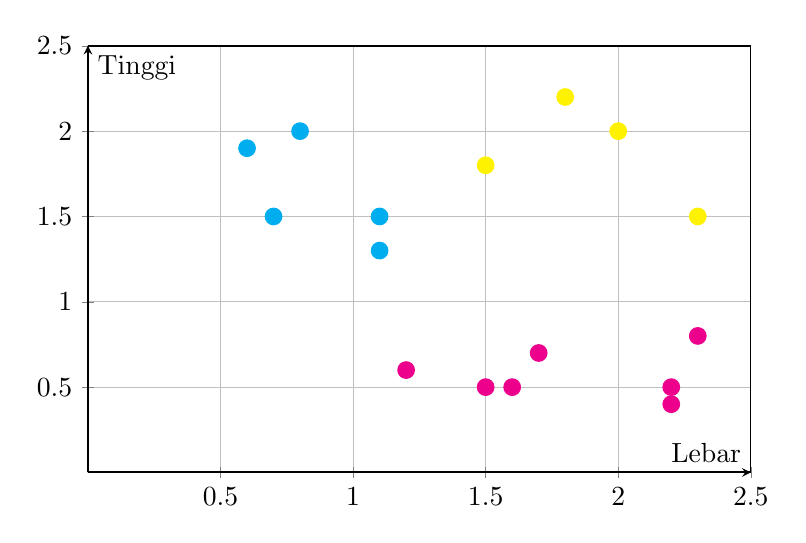
\begin{tikzpicture}
        \begin{axis}[
            xlabel=Lebar,
            ylabel=Tinggi,
            xmin=0, xmax=2.5,
            ymin=0, ymax=2.5,
            width=10cm,
            height=7cm,
            domain=-4:4,
            grid=both,
            samples=100,
            legend pos=south west,
            axis lines=middle, % Add this line to get the axes in the middle
        ]

        % Adding points
        \addplot[mark=*, color=cyan, mark size = 3] coordinates {(1.1,1.3)};
        \addplot[mark=*, color=cyan, mark size = 3] coordinates {(1.1,1.5)};
        \addplot[mark=*, color=cyan, mark size = 3] coordinates {(0.7,1.5)};
        \addplot[mark=*, color=cyan, mark size = 3] coordinates {(0.6,1.9)};
        \addplot[mark=*, color=cyan, mark size = 3] coordinates {(0.8,2)};
        \addplot[mark=*, color=magenta, mark size = 3] coordinates {(1.2,0.6)};
        \addplot[mark=*, color=magenta, mark size = 3] coordinates {(1.6,0.5)};
        \addplot[mark=*, color=magenta, mark size = 3] coordinates {(1.7,0.7)};
        \addplot[mark=*, color=magenta, mark size = 3] coordinates {(2.2,0.4)};
        \addplot[mark=*, color=magenta, mark size = 3] coordinates {(2.2,0.5)};
        \addplot[mark=*, color=magenta, mark size = 3] coordinates {(2.3,0.8)};
        \addplot[mark=*, color=magenta, mark size = 3] coordinates {(1.5,0.5)};
        \addplot[mark=*, color=yellow, mark size = 3] coordinates {(2,2)};
        \addplot[mark=*, color=yellow, mark size = 3] coordinates {(1.8,2.2)};
        \addplot[mark=*, color=yellow, mark size = 3] coordinates {(1.5,1.8)};
        \addplot[mark=*, color=yellow, mark size = 3] coordinates {(2.3,1.5)};


        % Draw frame
        \draw[black, thick] (rel axis cs:0,0) rectangle (rel axis cs:1,1);
        \end{axis}
    \end{tikzpicture}
    \caption{Grafik dari dataset pada Tabel \ref{tab:Dataset}. \textit{Cyan} adalah lemari, \textit{magenta} adalah buffet, dan kuning adalah wardrobe}
    \label{fig:plot dataset}
\end{figure}

Pada Gambar \ref{fig:plot dataset} terlihat bahwa terdapat jarak diantara ketiga kelas sehingga dataset dapat dikatakan \textit{linearly separable}.

\section{Metode yang Digunakan}

Penelitian dilakukan dengan mengembangkan model jaringan syaraf tiruan yang dilatih dengan dataset yang ada. Pengembangan jaringan syaraf tiruan dilakukan dengan bahasa pemrograman python versi 3.10.12 yang dijalankan pada \textit{Cloud Computing} Google Colaboratory. Dataset akan diproses terlebih dahulu dengan metode normalisasi \textit{minmax scalling}. Dataset yang telah dinormalisasi diteruskan ke lapisan berikutnya melalui \textit{forward bias} hingga mencapai lapisan keluaran. Lapisan keluaran kemudian digunakan untuk menghitung \textit{lost function} atau perhitungan error antara lapisan output dan label dari data yang diberikan. \textit{Lost function} yang digunakan adalah \textit{Mean Square Error} (MSE), nilai dari MSE ini seiring dengan pelatihan neural network akan berkurang dengan metode \textit{Gradient Descent}. Jaringan syaraf tiruan akan menggunakan jumlah \textit{hidden layer} yang bervariasi untuk melihat perubahan pada waktu komputasi dan akurasinya. Terdapat tiga model yang akan digunakan yaitu model pertama dengan satu hidden layer dengan variasi neuron-nya, model kedua dengan neuron yang sama namun dengan jumlah hidden layer yang bervariasi, dan model ketiga dengan jumlah bobot yang sama namun dengan jumlah hidden layer yang berbeda. Ketiga model akan menggunakan fungsi aktivasi \textit{step function} pada \textit{output layer}. Pelatihan model menggunakan metode \textit{gradient descent} untuk menurunkan nilai dari \textit{Mean Square Error} sebagai \textit{lost function}. Nilai dari bobot akan beradaptasi seiring dengan penurunan nilai \textit{Mean Square Error}.

\section{Alur Penelitian}

Penelitian ini dilakukan secara bertahap dengan alur seperti pada Gambar \ref{alur_penelitian}.
Studi literatur dilakukan pada awal penelitian untuk memahami konsep dan teori yang akan digunakan pada penelitian. Selanjutnya, dilakukan Pengembangan program jaringan syaraf tiruan dengan bahasa pemrograman python pada \textit{google colaboratory}. Setelah program dibuat, maka dilakukan pengujian untuk mengetahui apakah program berhasil atau tidak. Penelitian diakhiri dengan pengambilan data pengujian dan penyusunan laporan akhir.

\begin{figure}[H]
	\centering
	\resizebox{0.35\textwidth}{!}{%
		\tikzstyle{startstop} = [rectangle, rounded corners, minimum width=3cm, minimum height=1cm, text centered, draw=black, fill=red!30]
		\tikzstyle{analyze} = [rectangle, text width=5cm, minimum width=3cm, minimum height=1cm, text centered, draw=black, fill=orange!30]
		\tikzstyle{process} = [rectangle, text width=5cm, minimum width=3cm, minimum height=1cm, text centered, draw=black, fill=orange!30]
		\tikzstyle{decision} = [diamond, text width=1.5cm, minimum width=1cm, minimum height=1cm, text centered, draw=black, fill=green!30]
		\tikzstyle{arrow} = [thick,->,>=stealth]
		\begin{tikzpicture}[node distance=2cm]
			\node (start) [startstop] {Mulai};
			\node (input) [analyze, below of=start, yshift=0.5cm] {Studi Literatur};
                \node (process1) [process, below of=input, yshift=0.5cm]{Pengembangan \textit{class neural network} dengan python};
			\node (process2) [process, below of=process1, yshift=0.5cm] {Melakukan pengujian model};
			\node (decision) [decision, below of=process2, yshift=-0.2cm] {Berhasil?};
                \node (process3) [process, below of=decision, yshift=-0.4cm] {Pengujian dengan satu hidden layer dengan variasi jumlah neuron};
                \node (process4) [process, below of=process3, yshift=-0.4cm] {Pengujian dengan variasi jumlah hidden layer dengan jumlah neuron yang sama};
                \node (process5) [process, below of=process4, yshift=-0.4cm] {Pengujian dengan variasi jumlah hidden layer dengan jumlah bobot yang sama};
			\node (process6) [analyze, below of=process5, yshift=0.1cm] {Pengambilan data};
			\node (stop) [startstop, below of=process6, yshift=0.5cm] {Selesai};
			\draw [arrow] (start) -- (input);
			\draw [arrow] (input) -- (process1);
			\draw [arrow] (process1) -- (process2);
			\draw [arrow] (process2) -- (decision);
			\draw [arrow] (decision.south) -- node[anchor=west, pos=0.3] {Iya} (process3);
			\draw [arrow] (decision.west) -- node[anchor=south, pos=0.2] {Tidak} (-4,-6.7) -- (-4,-3) -- (process1.west);
                \draw [arrow] (process3) -- (process4);
                \draw [arrow] (process4) -- (process5);
                \draw [arrow] (process5) -- (process6);
                \draw [arrow] (process6) -- (stop);
		\end{tikzpicture}%
        }
	\caption{\textit{Flowchart} alur penelitian}
    \label{alur_penelitian}
\end{figure}

\subsection{Studi Literatur}
Studi literatur merupakan tahap awal pada penelitian agar dapat memahami lebih lanjut topik penelitian yang dilakukan. Studi literatur dilakukan dengan mengumpulkan materi dan referensi dari berbagai sumber seperti artikel, jurnal penelitian, forum, dan situs web.

\subsection{Pengembangan program jaringan syaraf tiruan dengan python}
Pengembangan program dilakukan pada \textit{Google Colaboratory} dengan menggunakan bahasa pemrograman python. Diagram alir dari program terlihat pada Gambar \ref{alur_program}

\begin{figure}[H]
	\centering
	\resizebox{0.35\textwidth}{!}{%
		\tikzstyle{startstop} = [rectangle, rounded corners, minimum width=3cm, minimum height=1cm, text centered, draw=black, fill=red!30]
		\tikzstyle{process} = [rectangle, text width=5cm, minimum width=3cm, minimum height=1cm, text centered, draw=black, fill=orange!30]
		\tikzstyle{decision} = [diamond, text width=1.5cm, minimum width=1cm, minimum height=1cm, text centered, draw=black, fill=green!30]
		\tikzstyle{arrow} = [thick,->,>=stealth]
		\begin{tikzpicture}[node distance=2cm]
			\node (start) [startstop] {Mulai};
			\node (process1) [process, below of=start, yshift=0.6cm] {Import Library};
                \node (process2) [process, below of=process1, yshift=0.6cm]{Akuisisi dan \textit{Pre processing data}};
			\node (process3) [process, below of=process2, yshift=0.5cm] {\textit{Pembuatan Class Neural Network}};
			\node (stop) [startstop, below of=process3, yshift=0.6cm] {Selesai};
			\draw [arrow] (start) -- (process1);
			\draw [arrow] (process1) -- (process2);
			\draw [arrow] (process2) -- (process3);
			\draw [arrow] (process3) -- (stop);
		\end{tikzpicture}%
        }
	\caption{Diagram alir program}
    \label{alur_program}
\end{figure}

\subsubsection{Import Library}

\begin{lstlisting}
    import numpy as np
    import pandas as pd
\end{lstlisting}

Import library digunakan untuk memasukan library yang dibutuhkan kedalam program. Library yang dibutuhkan adalah library numpy dan library pandas. Numpy digunakan untuk melakukan pengoperasian matriks, sedangkan pandas digunakan untuk mengambil sumber data yang berbentuk file csv.

\subsubsection{Akuisisi dan \textit{pre-processing} data}

Dataset pada Tabel \ref{tab:Dataset} tersebut masih dalam bentuk data mentah atau \textit{raw}. Data tersebut perlu diolah terlebih dahulu untuk memudahkan proses pelatihan. Beberapa pengolahan data yang diperlukan adalah pemberian label dan juga normalisasi data. Label dibutuhkan terutama pada algoritma \textit{supervised learning} seperti pada model ANN. Label ini disebut juga sebagai \textit{expected value} karena label ini yang diharapkan keluar dari model yang dilatih. Terdapat beberapa metode dalam pemberian label. \textit{One vs All} adalah metode yang akan digunakan. Data akan diberi nilai 1 pada label yang bersesuaian dan -1 pada label lainnya. Kemudian data tersebut dinormalisasikan dan dirubah skalanya. Normalisasi dilakukan dengan metode Minmax Scaling.

\begin{table}[H]
    \centering
    \begin{tabular}{||p{1em}|p{3em}|p{3em}|p{2em}|p{2em}|p{2em}||}
    \hline
       No & Lebar & Tinggi & $C_0$ & $C_1$ & $C_2$\\ [0.5ex]
        \hline\hline
        1 & 1.1 & 1.3 & 1 & -1 & -1\\ \hline 
        2 & 1.1 & 1.5 & 1 & -1 & -1\\ \hline	
        3 & 0.7 & 1.5 & 1 & -1 & -1\\ \hline	
        4 & 0.6 & 1.9 & 1 & -1 & -1\\ \hline	
        5 & 0.8 & 2 & 1 & -1 & -1\\ \hline	
        6 & 1.2 & 0.6 & -1 & 1 & -1\\ \hline	
        7 & 1.6 & 0.5 & -1 & 1 & -1\\ \hline	
        8 & 1.7 & 0.7 & -1 & 1 & -1\\ \hline	
        9 & 2.2 & 0.4 & -1 & 1 & -1\\ \hline	
        10 & 2.2 & 0.5 & -1 & 1 & -1\\ \hline	
        11 & 2.3 & 0.8 & -1 & 1 & -1\\ \hline	
        12 & 1.5 & 0.5 & -1 & 1 & -1\\ \hline
        13 & 2 & 2 & -1 & -1 & 1\\ \hline
        14 & 1.8 & 2.2 & -1 & -1 & 1\\ \hline	
        15 & 1.5 & 1.8 & -1 & -1 & 1\\ \hline	
        16 & 2.3 & 1.5 & -1 & -1 & 1\\ \hline
        \end{tabular}
    \caption{Dataset ukuran lebar dan tinggi dari lemari, buffet, dan wardrobe setelah diberi label}
    \label{tab:Dataset label}
\end{table}

Tabel \ref{tab:Dataset label} menunjukan bagaimana pemberian label dilakukan pada kelas lemari. Dimana $C_0$ diberikan nilai 1 sedangkan $C_1$ dan $C_2$ bernilai -1. Pada kelas buffet $C_1$ diberikan nilai 1 sedangkan $C_0$ dan $C_2$ bernilai -1. Hal tersebut dilakukan juga pada kelas Wardrobe. Oleh karena itu metode ini disebut \textit{One vs All}. Setelah dataset  diberikan label dengan metode \textit{One vs All}. Kemudian data disimpan kedalam \textit{Google Drive} dalam format csv.

\begin{lstlisting}
    from google.colab import drive
    drive.mount('/content/drive/')
    data = pd.read_csv('/content/drive/MyDrive/skripsi/data/datalemari(-1,1).csv')
    data.head()
\end{lstlisting}

Sumber data yang tersimpan pada \textit{Google Drive} perlu diakses agar dapat digunakan kedalam bahasa pemrograman \textit{python}. \textit{Google Drive} digunakan untuk memudahkan pengaksesan data oleh \textit{Google Colaboratory} karena masih dalam satu \textit{environment}. Kemudian Library Pandas digunakan untuk menyimpan data file csv menjadi bentuk \textit{DataFrame} pada python dengan cara mengisi lokasi dari file csv data pada perintah \textit{read\_csv}. Setelah data disimpan kedalam program selanjutnya data akan di \textit{pre-processing} terlebih dahulu dengan normalisasi \textit{minmax} dengan Persamaan \ref{eq:minmax}.

\begin{lstlisting}[language=C]
    def minmax_scaling (x_t):
        min = np.min(x_t)
        max = np.max(x_t)
        return ((x_t-min)/(max-min))
        
    X = minmax_scaling(data.iloc[:,:2].values.T)
    y = data.iloc[:,2:5].values.T
\end{lstlisting}

Fungsi diatas menggunakan Library numpy.max dan numpy.min untuk mencari nilai maksimum dan minimum pada array \textit{x\_t}. Kemudian  disimpan pada variabel X. Sedangkan variabel y akan menyimpan nilai label atau \textit{expected value} dari dataset.

\begin{table}[H]
    \centering
    \begin{tabular}{||p{1em}|p{3em}|p{3em}|p{2em}|p{2em}|p{2em}||}
    \hline
       No & Lebar & Tinggi & $C_0$ & $C_1$ & $C_2$\\ [0.5ex]
        \hline
        1 & 0.36 & 0.47 & 1 & -1 & -1\\ \hline 
        2 & 0.36 & 0.57 & 1 & -1 & -1\\ \hline	
        3 & 0.15 & 0.57 & 1 & -1 & -1\\ \hline	
        4 & 0.10 & 0.78 & 1 & -1 & -1\\ \hline	
        5 & 0.21 & 0.83 & 1 & -1 & -1\\ \hline	
        6 & 0.41 & 0.10 & -1 & 1 & -1\\ \hline	
        7 & 0.62 & 0.05 & -1 & 1 & -1\\ \hline	
        8 & 0.67 & 0.15 & -1 & 1 & -1\\ \hline	
        9 & 0.93 & 0.00 & -1 & 1 & -1\\ \hline	
        10 & 0.93 & 0.05 & -1 & 1 & -1\\ \hline	
        11 & 0.99 & 0.21 & -1 & 1 & -1\\ \hline	
        12 & 0.57 & 0.05 & -1 & 1 & -1\\ \hline
        13 & 0.83 & 0.83 & -1 & -1 & 1\\ \hline
        14 & 0.73 & 0.93 & -1 & -1 & 1\\ \hline	
        15 & 0.57 & 0.57 & -1 & -1 & 1\\ \hline	
        16 & 0.99 & 0.57 & -1 & -1 & 1\\ \hline
        \end{tabular}
    \caption{Dataset ukuran lebar dan tinggi dari lemari, buffet, dan wardrobe setelah normalisasi}
    \label{tab:Dataset normalisasi}
\end{table}

Table \ref{tab:Dataset normalisasi} menunjukan data telah diubah ukurannya menjadi rentang 0 hingga 1 setelah melalui proses normalisasi Minmax Scaling. Gambar \ref{fig:plot dataset normalisasi} menunjukkan plot kartesian dari Table \ref{tab:Dataset normalisasi}.

\begin{figure}[H]
    \centering
    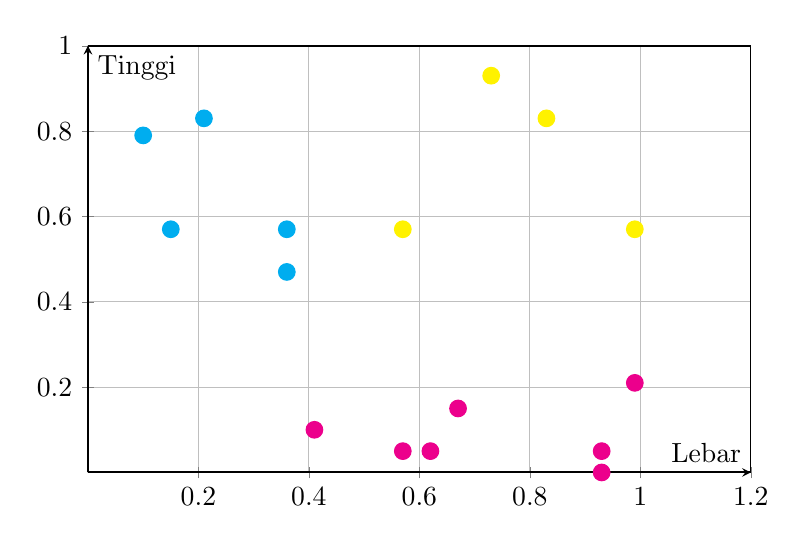
\begin{tikzpicture}
        \begin{axis}[
            xlabel=Lebar,
            ylabel=Tinggi,
            xmin=0, xmax=1.2,
            ymin=0, ymax=1,
            width=10cm,
            height=7cm,
            domain=-4:4,
            grid=both,
            samples=100,
            legend pos=south west,
            axis lines=middle, % Add this line to get the axes in the middle
        ]

        % Adding points
        \addplot[mark=*, color=cyan, mark size = 3] coordinates {(0.36,0.47)};
        \addplot[mark=*, color=cyan, mark size = 3] coordinates {(0.36,0.57)};
        \addplot[mark=*, color=cyan, mark size = 3] coordinates {(0.15,0.57)};
        \addplot[mark=*, color=cyan, mark size = 3] coordinates {(0.10,0.79)};
        \addplot[mark=*, color=cyan, mark size = 3] coordinates {(0.21,0.83)};
        \addplot[mark=*, color=magenta, mark size = 3] coordinates {(0.41,0.10)};
        \addplot[mark=*, color=magenta, mark size = 3] coordinates {(0.62,0.05)};
        \addplot[mark=*, color=magenta, mark size = 3] coordinates {(0.67,0.15)};
        \addplot[mark=*, color=magenta, mark size = 3] coordinates {(0.93,0.00)};
        \addplot[mark=*, color=magenta, mark size = 3] coordinates {(0.93,0.05)};
        \addplot[mark=*, color=magenta, mark size = 3] coordinates {(0.99,0.21)};
        \addplot[mark=*, color=magenta, mark size = 3] coordinates {(0.57,0.05)};
        \addplot[mark=*, color=yellow, mark size = 3] coordinates {(0.83,0.83)};
        \addplot[mark=*, color=yellow, mark size = 3] coordinates {(0.73,0.93)};
        \addplot[mark=*, color=yellow, mark size = 3] coordinates {(0.57,0.57)};
        \addplot[mark=*, color=yellow, mark size = 3] coordinates {(0.99,0.57)};


        % Draw frame
        \draw[black, thick] (rel axis cs:0,0) rectangle (rel axis cs:1,1);
        \end{axis}
    \end{tikzpicture}
    \caption{Grafik dari dataset setelah melalui Minmax Scaling. \textit{Cyan} adalah lemari, \textit{magenta} adalah buffet, dan kuning adalah wardrobe}
    \label{fig:plot dataset normalisasi}
\end{figure}


\subsubsection{Pembuatan \textit{Class Neural Network}}

\begin{figure}[H]
    \centering
    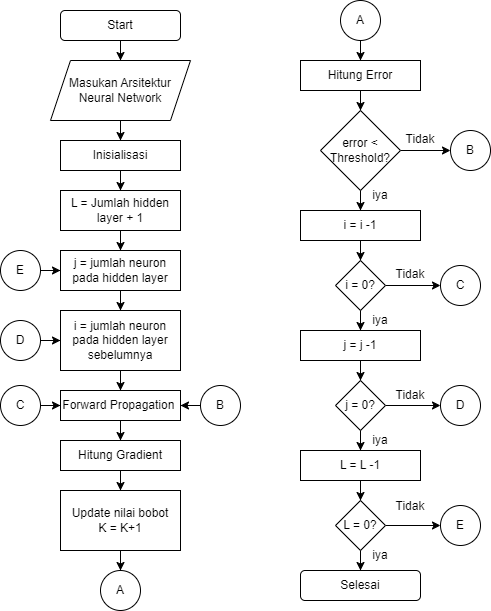
\includegraphics[width=9cm]{contents/chapter-3/Diagram Alir class.drawio.png}
    \caption{Diagram Alir Class Neural Network}
    \label{fig:Flowchart Class}
\end{figure}

Pembuatan \textit{class} ditunjukan agar dengan satu \textit{source code} dapat dilakukan percobaan dengan nilai jaringan tersembunyi yang dapat dirubah-ubah sesuai dengan model yang diinginkan. Pembuatan kelas juga dapat membantu penulis dalam melakukan perbaikan pada program. Diagram alir dari \textit{Class Neural Network} ditunjukkan pada Gambar \ref{fig:Flowchart Class}. 
\begin{lstlisting}
    def __init__(self, input_size, hidden_size, output_size, weight_init=0.5):
        self.input_size = input_size
        self.hidden_size = hidden_size
        self.output_size = output_size
        self.num_layers = np.concatenate(([input_size], hidden_size, [output_size]))
        self.L = len(self.num_layers)-1
        self.weight = {}
        self.Y = {}
        self.F = {}
        self.delta = {}
        self.dJ_dF = {}
        self.dF_dY = {}
        self.dY_dF = {}
        self.dJ_dw = {}
        self.t = 0
        self.d2J_dw2 = {}
        self.accuracy = []
        self.mse = []

        if weight_init == 'random':
            for l in range(0, self.L):
                self.weight[f'w{l}'] = np.random.rand(self.num_layers[l+1], self.num_layers[l]+1)
                self.dJ_dw[f'{l}'] = np.array([])

        else:
            for l in range(0, self.L):
                self.weight[f'w{l}'] = weight_init * np.ones((self.num_layers[l+1], self.num_layers[l]+1))
                self.dJ_dw[f'{l}'] = np.array([])
\end{lstlisting}

Inisialisasi adalah fungsi yang pertama kali dijalankan ketika \textit{Class Neural Network} dipanggil. Inisialisasi akan membuat variabel-variabel yang diperlukan oleh neural network. Termasuk didalamnya adalah bobot awal yang akan digunakan selama pelatihan. Sebagai contoh pada Gambar \ref{fig:2.2 Jaringan Syaraf Tiruan} jaringan tersebut memiliki satu \textit{hidden layer} sehingga jaringan memiliki dua buah bobot maka L akan bernilai 2, bobot tersebut adalah $W^1$ dan $W^2$.

\begin{equation}
    W^1 = 
    \begin{bmatrix}
        W^1_{0,0} & W^1_{0,1} & W^1_{0,2} \\
        W^1_{1,0} & W^1_{1,1} & W^1_{1,2} \\
        W^1_{2,0} & W^1_{2,1} & W^1_{2,2}
    \end{bmatrix}
     W^2 = 
    \begin{bmatrix}
        W^2_{0,0} & W^2_{0,1} & W^2_{0,2} \\
        W^2_{1,0} & W^2_{1,1} & W^2_{1,2} \\
        W^2_{2,0} & W^2_{2,1} & W^2_{2,2}
    \end{bmatrix}
\end{equation}

\begin{equation}
    W^1 = W^2 =  
    \begin{bmatrix}
        1 & 0 & 0 \\
        0.5 & 0.5 & 0.5 \\
        0.5 & 0.5 & 0.5
    \end{bmatrix}
    \label{eq:bobot awal}
\end{equation}

Setelah dibuat variabel untuk bobot maka langkah selanjutnya adalah dengan menentukan nilai bobot awal. Bobot awal ini umumnya dideklarasikan dengan suatu fungsi random. Namun karena fokus pada penelitian ini adalah jumlah dari hidden layer, maka nilai bobot akan dibuat sama, yaitu baris pertama akan bernilai 1 untuk mendistribusikan nilai bias. Kemudian baris lainnya akan bernilai 0.5 sama seperti pada persamaan \ref{eq:bobot awal}. 

\begin{lstlisting}
    def ForwardPropagation(self, X):
        self.X = np.append(np.ones((1, self.N), X, axis = 0)

        for l in range (0, self.L):
            if l == 0 :
                self.Y[f'{l}'] = np.dot(self.weight['w0'], self.X)
                self.F[f'{l}'] = self.tanh(self.Y[f'{l}'])
                self.F[f'{l}'] = np.append(np.ones((1,self.N)), self.F[f'{l}'], axis = 0)
            elif l == len(self.hidden_size):
                self.Y[f'{l}'] = np.dot(self.weight[f'w{l}'], self.F[f'{l-1}'])
                self.F[f'{l}'] = self.tanh(self.Y[f'{l}'])
                self.Y_out = self.Y[f'{l}']
                self.F_out = self.F[f'{l}']
                self.F_step = self.step_function(self.F[f'{l}'])
            else :
                self.Y[f'{l}'] = np.dot(self.weight[f'w{l}'], self.F[f'{l-1}'])
                self.F[f'{l}'] = self.tanh(self.Y[f'{l}'])
                self.F[f'{l}'] = np.append(np.ones((1,self.N)), self.F[f'{l}'], axis = 0)
        return
\end{lstlisting}

Setelah proses inisialisasi selesai dan semua variabel yang diperlukan sudah dibuat. Langkah selanjutnya adalah dengan melakukan \textit{Forward Porpagation} dengan menggunakan Persamaan \ref{eq: 2.8}. Setelah \textit{forward propagation} dilakukan hingga mencapai layer terakhir. Sinyal keluaran pada layer terakhir disebut juga sebagai \textit{predicted value}. \textit{Predicted value} ini bersamaan dengan \textit{expected value} dimasukkan kedalam \textit{lost function} MSE sebagai parameter \textit{error} dari model. Umumnya pada awal pelatihan nilai dari \textit{lost function} akan cukup tinggi. Semakin kecil \textit{lost function} semakin baik pula modelnya. Untuk menurunkan nilai \textit{lost function} dapat menggunakan \textit{Gradient descent} pada persamaan \ref{eq: 2.8}. Yaitu dengan menggunakan turunan \textit{lost function} terhadap parameter yang ingin dilatih. Karena dataset yang digunakan cukup kecil maka seluruh data akan digunakan dan disebut dengan \textit{stocasthic gradient descent}. berikut persamaan \ref{eq:fx'} dan \ref{eq:fx''}:

\begin{equation}
    \frac{d\text{MSE}}{dw^l_{(j,i)}}=\frac{d\frac{1}{N} \sum_{n=1}^{N} (d_n-y_n)^2}{dw^l_{(j,i)}}
    \label{eq:fx'}
\end{equation}
\begin{equation}
    \frac{d^2\text{MSE}}{d(w^l_{(j,i)})^2}=\frac{d^2\frac{1}{N} \sum_{n=1}^{N} (d_n-y_n)^2}{d(w^l_{(j,i)})^2}
    \label{eq:fx''}
\end{equation}

Dimana $w^l_{(j,i)}$ adalah bobot ke-l, yang terhubung dengan neuron j dan neuron i, $l=1, 2, ...,L$, $d_n$ adalah \textit{expected value} ke-n atau label ke-n, dan $y_n$ adalah \textit{predicted value} ke-n. Setelah mendapatkan gradiennya dengan Persamaan \ref{eq:fx'} dan Persamaan \ref{eq:fx''} nilai tersebut dimasukkan untuk memperbaharui bobot $w^l_{(j,i)}$. Dengan menggunakan aturan rantai maka penggunaannya diterapkan pada fungsi update seperti berikut :

\begin{lstlisting}
    def update(self, y):
        n = self.X.shape[1]

        for l in range(self.L, -1, -1):
            if l == len(self.hidden_size):
                self.dY_dY[f'{l}'] = self.weight[f'w{l}']
                self.delta[f'{l}'] = (-2 / n)  * (y-self.Y[f'{l}'])
                self.dJ_dw[f'{l}'] = np.dot(self.delta[f'{l}'], self.Y[f'{l-1}'].T)
                temp = self.delta[f'{l}']

                self.d2J_dw2[f'{l}'] = (2 / n) * np.sum(self.Y[f'{l-1}']**2, axis=1)
                self.d2J_dw2[f'{l}'] = np.outer(np.ones(self.output_size), self.d2J_dw2[f'{l}'])
                temp_2 = (2 / n) * np.sum(self.weight[f'w{l}']**2, axis=0)

            elif l == 0:
                self.delta[f'{l}'] = np.dot(self.dY_dY[f'{l+1}'].T, temp)
                self.dJ_dw[f'{l}'] = np.dot(self.delta[f'{l}'], self.X.T)

                self.d2J_dw2[f'{l}'] = np.outer(temp_2[:, np.newaxis], np.sum(self.X**2, axis =1)[np.newaxis, :])

            else:
                self.dY_dY[f'{l}'] = self.weight[f'w{l}']
                self.delta[f'{l}'] = np.dot(self.dY_dY[f'{l+1}'].T, temp)
                self.dJ_dw[f'{l}'] = np.dot(self.delta[f'{l}'], self.Y[f'{l-1}'].T)
                temp = self.delta[f'{l}']

                self.d2J_dw2[f'{l}'] = np.outer(temp_2[:, np.newaxis], np.sum(self.Y[f'{l-1}']**2, axis=1)[np.newaxis, :])
                temp_2 = np.dot(temp_2, self.weight[f'w{l}']**2)

        return
\end{lstlisting}

Setelah mendapatkan \textit{gradient} langkah selanjutnya adalah \textit{backpropagation} yaitu dengan mendistribusikan \textit{gradient} tersebut ke semua bobot yang ada dan melakukan pembaharuan bobot. Pembaharuan bobot menggunakan Persamaan \ref{eq:pembaharuan bobot}. Pembaharuan bobot dilakukan satu persatu yaitu dimulai dengan bobot terdepan yaitu bobot $w^l_{j,i}$. Pelatihan dilakukan pada satu bobot tersebut secara berulang hingga memenuhi kriteria \textit{threshold} pada \textit{relative error}, jika syarat sudah terpenuhi pelatihan pada bobot tersebut berhenti dan dilanjutkan pada bobot selanjutnya. Hal ini dilakukan berulang hingga semua bobot telah dilatih atau jika nilai \textit{predicted value} sudah serupa dengan nilai \textit{expected value}. Penggunaan $i, j,$ dan $l$ untuk memastikan agar semua bobot disetiap layer telah melalui proses pelatihan. Sedangkan $t$ adalah banyak iterasi yang dilakukan karena tiap bobot akan melakukan jumlah pelatihan yang berbeda. $t$ akan digunakan untuk membandingkan waktu komputasi yang dilaksanakan. Penggunaan algoritam tersebut akan disimpan pada fungsi \textit{backpropagation} didalam \textit{class Neural Network} seperti berikut:

\begin{lstlisting}
    def Backpropagation(self, X, y, learning_rate=0.1):
        self.ForwardPropagation(X)
        break_all_loop = False
        for l in range(self.L, -1, -1):
          for j in range(self.num_layers[w+1]):
            for i in range(self.num_layers[w]):
              while True:
                self.update(y)
                self.t +=1

                self.accuracy.append(self.accuracy_func(y, self.F))
                self.mse.append(self.mse_func(y, self.Y_out))

                delta_t = learning_rate * (self.dJ_dw[f'{l}'][j, i]/self.d2J_dw2[f'{l}'][j,i])
                w_n = self.weight[f'w{l}'][j, i] - delta_t

                error = self.error(w_n, self.weight[f'w{l}'][j, i])

                self.weight[f'w{l}'][j, i] = w_n
                self.ForwardPropagation(X)

                if np.sum(np.abs(y-self.F)) == 0:
                  self.accuracy.append(self.accuracy_func(y, self.F))
                  self.mse.append(self.mse_func(y, self.Y_out))
                  break_all_loop = True
                  break
                if error < 0.1 :
                  break

              if break_all_loop == True :
                break
            if break_all_loop == True :
              break
          if break_all_loop == True :
            break

        return
\end{lstlisting}

\subsection{Pengujian program jaringan syaraf tiruan}
Pengujian program jaringan syaraf tiruan dilakukan untuk mengetahui apakah program sudah sesuai dengan perintah yang diharapkan. Salah satu faktor penentu program tersebut telah berjalan dengan baik adalah dengan memperhatikan nilai \textit{lost function}-nya. Pelatihan jaringan syaraf tiruan pada program yang dibuat menggunakan metode \textit{gradient descent}, sehingga nilai dari \textit{lost function} dari program yang benar akan berkurang seiring dengan bertambahnya iterasi pada model tersebut.

\subsection{Pengujian dengan satu hidden layer dengan variasi jumlah neuron}
\begin{lstlisting}
    nn1 = {}
    nn1_mse_iterasi = {}
    nn1_accuracy_iterasi = {}
    for h_n in range (1, 11):
      print(f'Hidden Neuron{h_n}')
      nn1[f'{h_n}'] = NeuralNetwork(2, [h_n], 3, weight_init=0.5)
      nn1[f'{h_n}'].Backpropagation(X, y)
      nn1_mse_iterasi[f'{h_n}'] = []
      nn1_accuracy_iterasi[f'{h_n}'] = []
      for t in range (1, 10000):
        old_mse=nn1[f'{h_n}'].mse[-1]
        nn1_mse_iterasi[f'{h_n}'].append(old_mse)
        nn1_accuracy_iterasi[f'{h_n}'].append(nn1[f'{h_n}'].accuracy[-1])
        nn1[f'{h_n}'].Backpropagation(X, y)
        nn1[f'{h_n}'].ForwardPropagation(X)
        new_mse=nn1[f'{h_n}'].mse[-1]
        if new_mse == old_mse :
          print(f'error epoch ke-{t} :',np.sum((y-nn1[f'{h_n}'].Y_out)**2)/16)
          break
        if t % 100 == 0 :
          print(f'error epoch ke-{t} :',np.sum((y-nn1[f'{h_n}'].Y_out)**2)/16)
        if np.sum(np.abs(y-nn1[f'{h_n}'].F)) == 0:
          nn1_mse_iterasi[f'{h_n}'].append(new_mse)
          nn1_accuracy_iterasi[f'{h_n}'].append(nn1[f'{h_n}'].accuracy[-1])
          print(f'error epoch ke-{t} :',np.sum((y-nn1[f'{h_n}'].Y_out)**2)/16)
          break
\end{lstlisting}

Pada \textit{Source Code} program akan membuat \textit{Class Neural Network} dengan satu hidden layer namun dengan hidden neuron yang bervariasi. Variasi hidden neuron dilakukan dari 1 hingga 10 hidden neuron. Didalam \textit{Source Code} tersebut juga menyimpan beberapa variabel yang akan dianalisis lebih lanjut seperti nilai dari MSE dan juga akurasinya pada iterasi ke $t$.

\subsection{Pengujian dengan variasi jumlah hidden layer dengan jumlah neuron yang sama}

\begin{lstlisting}
    nn_vhl = {}
    nn_vhl_mse_iterasi = {}
    nn_vhl_accuracy_iterasi = {}
    for h_n in range (3, 7):
        start_hidden_layers = 1
        last_hidden_layers = 4
        hidden_neuron = []
        for h_l in range (start_hidden_layers, last_hidden_layers+1):
            print(f'number of hidden layer : {h_l}')
            print(f'number of neuron each hidden layer : {h_n}')
            hidden_neuron.append(h_n)
            nn_vhl[f'{h_n}{h_l}'] = NeuralNetwork(2, hidden_neuron, 3, weight_init= 0.3)
            nn_vhl[f'{h_n}{h_l}'].backward(X, y)
            nn_vhl_mse_iterasi[f'{h_n}{h_l}'] = []
            nn_vhl_accuracy_iterasi[f'{h_n}{h_l}'] = []
            for i in range (10000):
            old_mse = nn_vhl[f'{h_n}{h_l}'].mse[-1]
            nn_vhl_mse_iterasi[f'{h_n}{h_l}'].append(old_mse)
            nn_vhl_accuracy_iterasi[f'{h_n}{h_l}'].append(nn_vhl[f'{h_n}{h_l}'].accuracy[-1])
            nn_vhl[f'{h_n}{h_l}'].backward(X, y, learning_rate=0.1)
            nn_vhl[f'{h_n}{h_l}'].forward(X)
            new_mse = nn_vhl[f'{h_n}{h_l}'].mse[-1]
            nn_vhl[f'{h_n}{h_l}'].backward(X, y, 0.1)
            nn_vhl[f'{h_n}{h_l}'].forward(X)
            if new_mse == old_mse :
              print(f'error epoch ke-{i} :',np.sum((y-nn_vhl[f'{h_n}{h_l}'].Y_out)**2)/16)
              break
            if i % 100 == 0 :
              print(f'error epoch ke-{i} :',np.sum((y-nn_vhl[f'{h_n}{h_l}'].Y_out)**2)/16)
            if np.sum(np.abs(y-nn_vhl[f'{h_n}{h_l}'].F)) == 0:
              nn_vhl_mse_iterasi[f'{h_n}{h_l}'].append(new_mse)
              nn_vhl_accuracy_iterasi[f'{h_n}{h_l}'].append(nn_vhl[f'{h_n}{h_l}'].accuracy[-1])
              print(f'error epoch ke-{i} :',np.sum((y-nn_vhl[f'{h_n}{h_l}'].Y_out)**2)/16)
              break
\end{lstlisting}

Pada pengujian ini yaitu dengan melakukan variasi jumlah hidden layer degan jumlah neuron yang sama pada tiap hidden layernya. variasi jumlah hidden layer dilakukan dari satu hidden layer hingga empat hidden layer. Sedangkan jumlah Hidden Neuron yang dibuat sama dilakukan dari 3 Hidden Neuron hingga 6 Hidden Neuron. Variabel $h\_l$ akan digunakan untuk menyimpan hidden layer yang digunakan. Variabel $h\_n$ digunakan untuk menyimpan jumlah hidden neuron yang digunakan

\subsection{Pengujian dengan variasi jumlah hidden layer dengan jumlah bobot yang sama}

Pada pengujian ini diperlukan jumlah bobot yang sesuai untuk bisa digunakan pada jumlah hidden layer yang bervariasi. Dengan menggunakan faktor-faktor darijumlah bobot yang akan digunakan, ditemukan bobot yang dapat digunakan adalah 72, 105, 144, dan 189.

\begin{lstlisting}
    nn_34643 = NeuralNetwork(2, [4, 6, 4], 3, weight_init=0.3)
    nn_34643_mse_iterasi = []
    nn_34643_accuracy_iterasi = []
    nn_34643.Backpropagation(X, y, learning_rate=0.1)
    for i in range (1, 10000):
      old_mse=nn_34643.mse[-1]
      nn_34643_mse_iterasi.append(old_mse)
      nn_34643_accuracy_iterasi.append(nn_344443.accuracy[-1])
      nn_34643.Backpropagation(X, y, learning_rate=0.1)
      nn_34643.ForwardPropagation(X)
      new_mse = nn_34643.mse[-1]
      if new_mse == old_mse :
        print(f'error epoch ke-{i} :',np.sum((y-nn_34643.Y_out)**2)/16)
        break
      if i % 100 == 0 :
        print(f'error epoch ke-{i} :',np.sum((y-nn_34643.Y_out)**2)/16)
      if np.sum(np.abs(y-nn_34643.F)) == 0:
        nn_34643_mse_iterasi.append(new_mse)
        nn_34643_accuracy_iterasi.append(nn_34643.accuracy[-1])
        print(f'error epoch ke-{i} :',np.sum((y-nn_34643.Y_out)**2)/16)
        break
\end{lstlisting}
Pada \textit{Source Code} diatas menunjukkan bagaimana untuk mencari jumlah bobot yang dapat digunakan. Untuk jumlah bobot sebesar 72 maka arsitektur yang akan dibuat adalah 3-4-6-4-3, 3-6-6-3, dan 3-12-3. Untuk jumlah bobot sebesar 105 maka arsitektur yang akan dibuat adalah 3-5-5-5-5-3 dan 3-7-4-8-3. Untuk jumlah bobot sebesar 144 maka arsitektur yang akan dibuat adalah 3-6-6-6-6-3, 3-3-21-3-3, 3-6-14-3, dan 3-24-3, Untuk jumlah bobot sebesar 72 maka arsitektur yang akan dibuat adalah 3-7-7-7-7-3, 3-10-6-11-3, dan 3-6-19-3. Dengan Kombinasi tersebut maka akan dihasilkan jumlah bobot yang sama.

\subsection{Pengambilan data}
Setelah program sudah diyakini benar maka langkah selanjutnya adalah mengambil data yang ingin dianalisis. Dalam penelitian ini data yang diambil adalah jumlah \textit{hidden layer}, akurasi, dan waktu komputasi.
\chapter{Hasil dan Pembahasan}
\section{Hasil Pengujian dengan satu hidden layer dengan variasi jumlah neuron}
\begin{figure}[H]
    \centering
    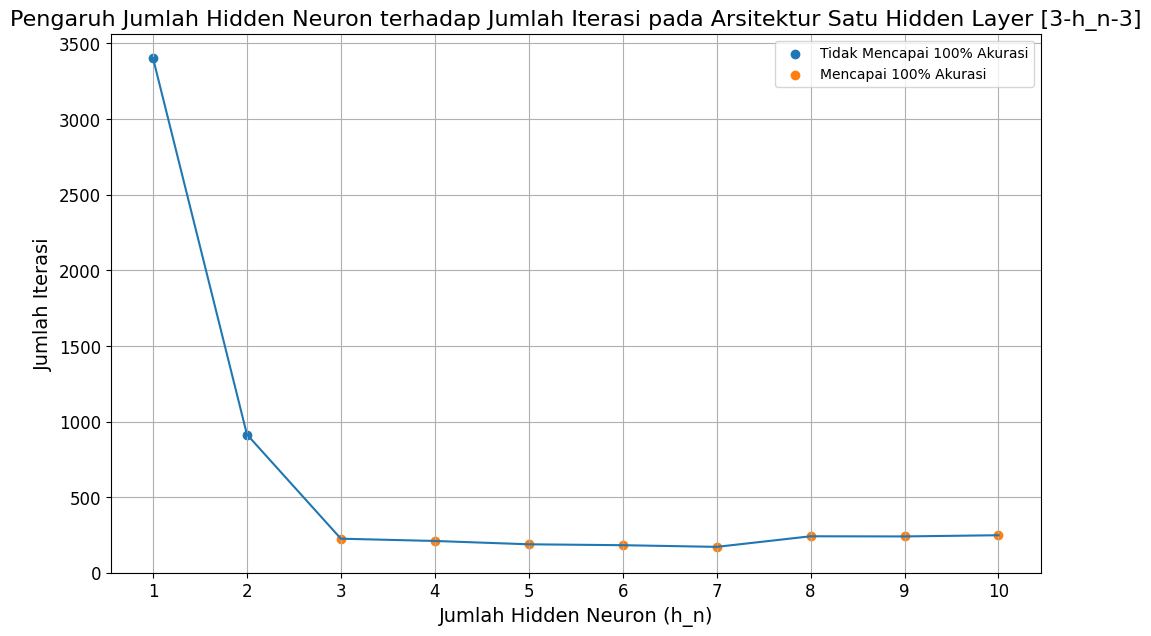
\includegraphics[width=14cm]{contents/chapter-4/1.png}
    \caption{Grafik akurasi terhadap jumlah iterasi}
    \label{fig:Plot VHN Iterasi}
\end{figure}

Pada gambar \ref{fig:Plot VHN Iterasi} terlihat pengaruh jumlah hidden neuron pada 1 hidden layer dengan arsitektur [3-h\_n-3]. Terlihat pada konfigurasi dengan 1 dan 2 hidden neuron tidak mencapai akurasi 100\%. Sedangkan pada konfigurasu 3 hingga 10 hidden neuron berhasil mencapai 100\% akurasi. Untuk melihat trend nya dapat menggunakan \textit{Polynomial Curve Fit}.

\begin{figure}[H]
    \centering
    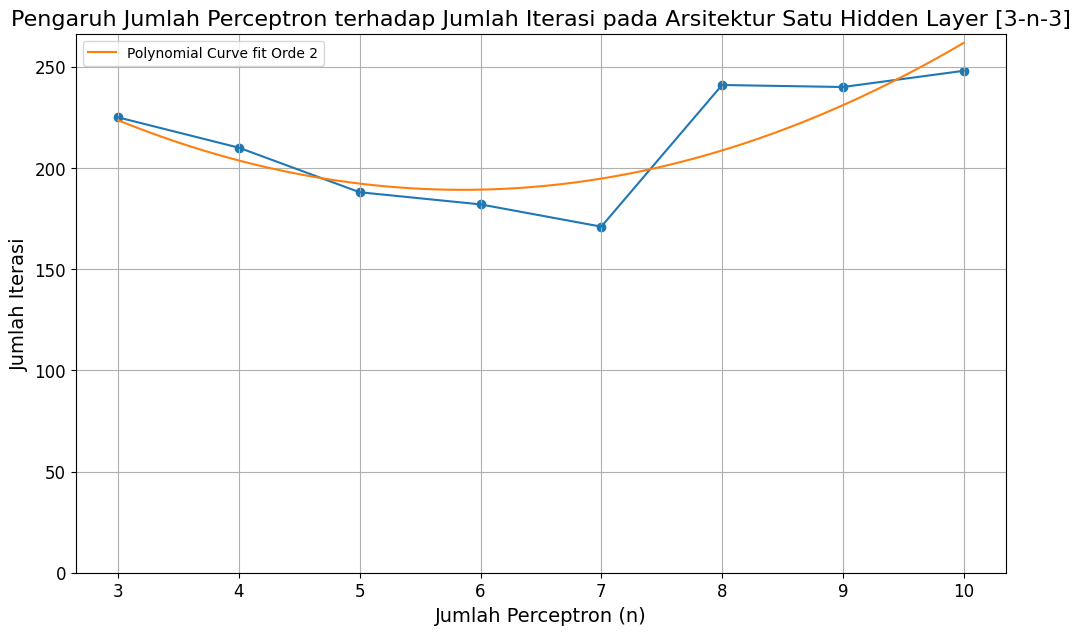
\includegraphics[width=14cm]{contents/chapter-4/2.png}
    \caption{Grafik akurasi terhadap jumlah iterasi}
    \label{fig:Plot VHN Iterasi 2}
\end{figure}

Pada gambar \ref{fig:Plot VHN Iterasi 2} akan difokuskan pada jaringan yang berhasil mencapai 100\% akurasi. Terlihat dengan menggunakan \textit{Polynomial Curve Fit} orde 2 bahwa iterasi turun seiring degan penambahan jumlah hidden neuron hingga titik tertentu, kemudian meningkat kembali.

\begin{figure}[H]
    \centering
    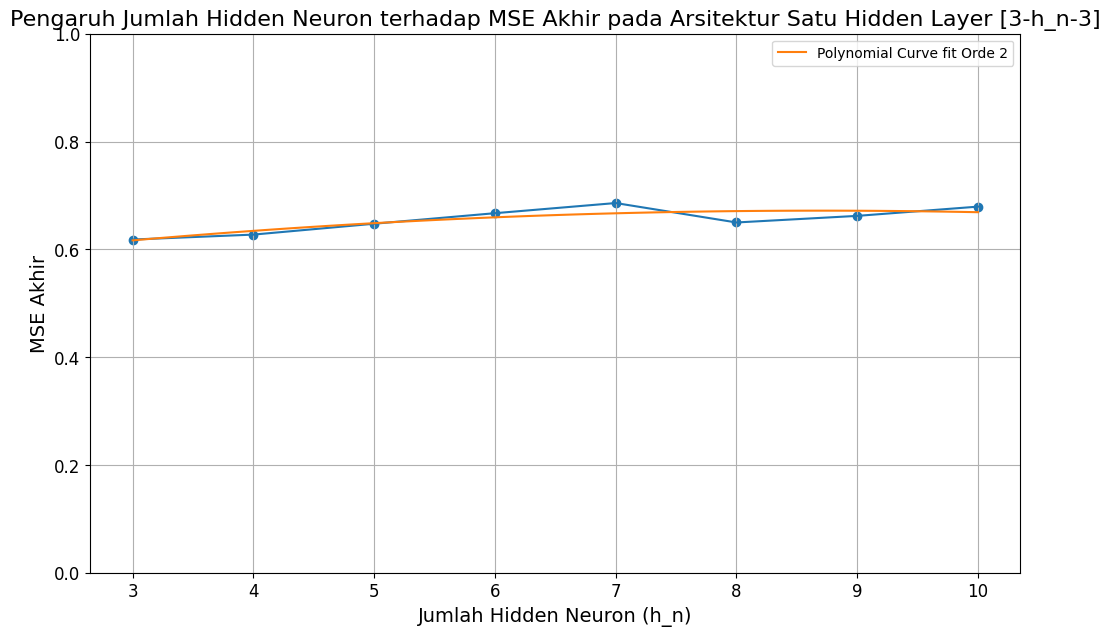
\includegraphics[width=14cm]{contents/chapter-4/3.png}
    \caption{Grafik akurasi terhadap jumlah iterasi}
    \label{fig:Plot VHN MSE}
\end{figure}

Pada gambar \ref{fig:Plot VHN MSE} terlihat bahwa nilai MSE akhir meningkat seiring dengan penurunan jumlah iterasi yang diperlukan untuk mencapai 100\% akurasi. Hal ini akan lebih terlihat jika kedua plot dibuat dalam satu figur seperti pada Gambar \ref{fig:Plot VHN MSE Akurasi}.

\begin{figure}[H]
    \centering
    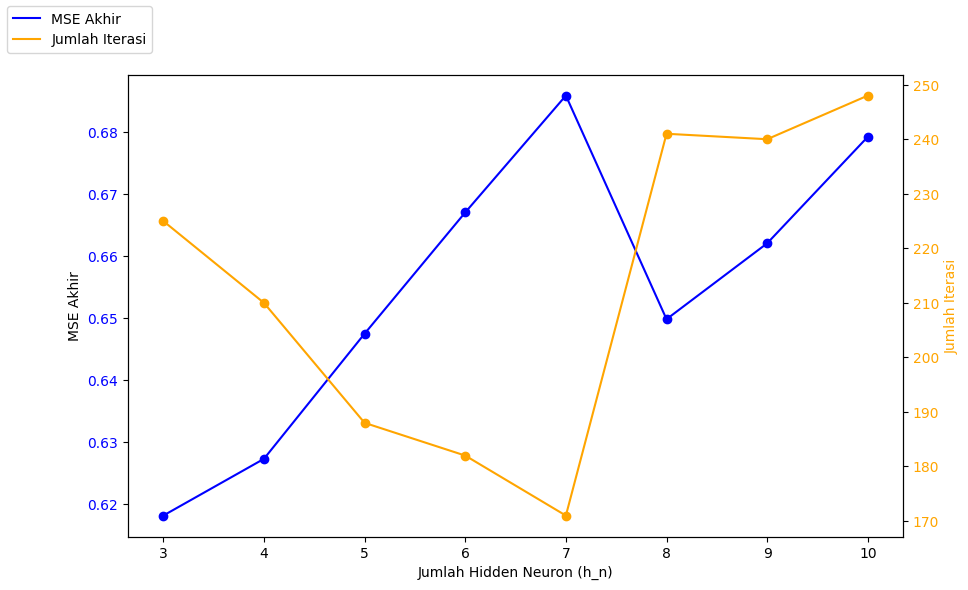
\includegraphics[width=14cm]{contents/chapter-4/4.png}
    \caption{Grafik akurasi terhadap jumlah iterasi}
    \label{fig:Plot VHN MSE Akurasi}
\end{figure}

\section{Hasil Pengujian  dengan variasi jumlah hidden layer dengan jumlah neuron yang
sama}

Pelatihan dilakukan dengan jumlah hidden layer yang bervariasi mulai dari 1 hingga 4 hidden layer dan 3 hingga 6 Hidden Neuron. Nilai awal bobot dibuat serupa untuk semua variasi yaitu sesuai dengan Persamaan \ref{eq:bobot awal}. Nilai Threshold dibuat 0.1 dan nilai \textit{learning rate} dibuat 0.1. Detail pelatihan lebih lanjut dijelaskan pada Halaman \pageref{fig:Flowchart Class}. Data hasil yang diambil berupa grafik jumlah Hidden Neuron dengan jumlah iterasinya.

\begin{figure}[H]
    \centering
    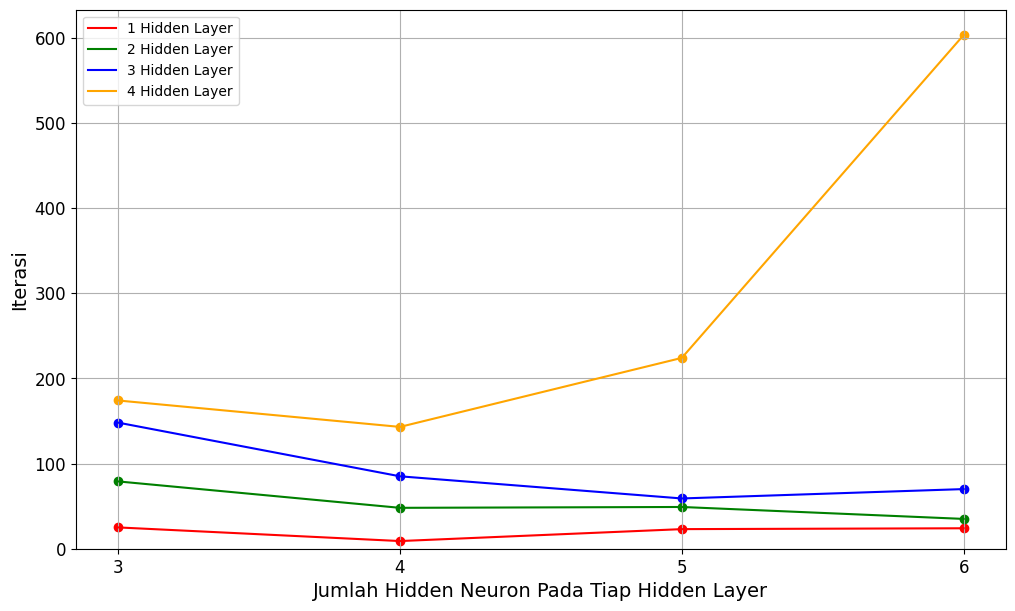
\includegraphics[width=14cm]{contents/chapter-4/5.png}
    \caption{Grafik akurasi terhadap jumlah iterasi}
    \label{fig:Grafik Akurasi}
\end{figure}

Pada Gambar \ref{fig:Grafik Akurasi} terlihat bahwa semua konfigurasi dari 1 hidden layer hingga 4 hidden layer mencapai 100\% akurasi. Terlihat bahwa semakin banyak \textit{hidden layer} semakin banyak pula iterasi yang diperlukan. Dan dengan konfigurasi 4 \textit{Hidden Layer} dengan 6 \textit{Hidden Neuron} di setiap \textit{Hidden layer}nya memiliki jumlah iterasi terbanyak. Pada konfigurasi tersebut akan memiliki 144 bobot. 

\section{Hasil Pengujian dengan variasi jumlah hidden layer dengan jumlah bobot yang
sama}

Pengujian menggunakan bobot yang sama dengan variasi jumlah Hidden Layer yang berbeda. Pemilihan bobot yang benar diperlukan karena tidak semua jumlah bobot dapat dibuat pada beberapa jumlah \textit{Hidden layer} tertentu.

\begin{figure}[H]
    \centering
    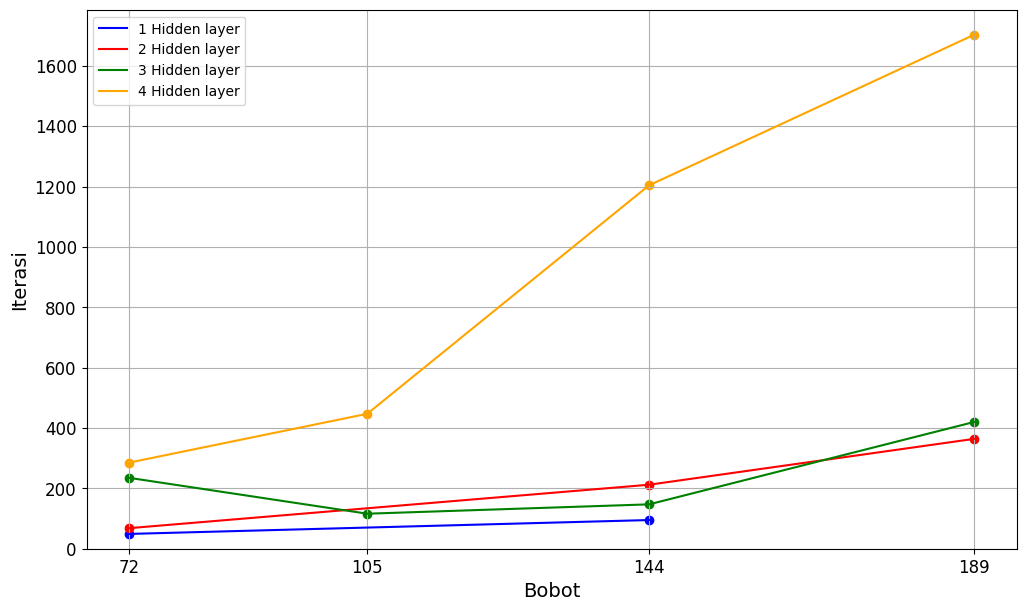
\includegraphics[width=14cm]{contents/chapter-4/6.png}
    \caption{Grafik akurasi terhadap jumlah iterasi}
    \label{fig:Grafik Akurasi 1}
\end{figure}

Sebagai contoh adalah pada Gambar \ref{fig:Grafik Akurasi 1}, terlihat bahwa bobot 105 tidak memiliki konfigurasi pada 1 dan 2 Hidden layer. Pada Jumlah bobot 189 juga tidak ditemukan konfigurasi untuk 1 Hidden layer. Berdasarkan gambar tersebut 4 hidden layer selalu memiliki jumlah iterasi terbanyak dibanding dengan konfigurasi \textit{Hidden Layer} lebih sedikit. Sedangkan dengan  konfigurasi 3 \textit{hidden layer} memiliki jumlah iterasi yang lebih tinggi dari 1 atau 2 hidden layer kecuali pada jumlah bobot 144 dan selalu lebih rendah dari 4 jumlah hidden layer. 

\chapter{Kesimpulan dan Saran}

\section{Kesimpulan}

Berdasarkan penelitian yang telah dilakukan, dapat ditarik beberapa kesimpulan sebagai berikut:
\begin{enumerate}
    \item Penggunaan arsitektur dengan 1 hidden layer menunjukkan bahwa semakin banyak neuron pada hidden layer semakin sedikit iterasi yang diperlukan sampai pada 7 hidden neuron dan meningkat kembali.
    \item Penggunaan arsitektur dengan jumlah neuron yang sama pada tiap layer menunjukkan semakin banyak hidden layer semakin lama pula waktu iterasi yang dibutuhkan. Hal ini terjadi pada konfigurasi 3, 4, 5, dan 6 hidden layer.
    \item Penggunaan arsitektur dengan jumlah bobot yang sama menunjukkan 4 hidden layer selalu memiliki waktu komputasi yang lebih lama dibandingkan dengan jumlah hidden layer yang lebih sedikit. Satu hidden layer selalu memiliki waktu komputasi yang lebih sedikit dibanding dengan jumlah hidden layer lebih banyak. 
    \item Penggunaan arsitektur dengan jumlah hidden neuron yang lebih sedikit dari neuron pada layer masukan selalu gagal mencapai 100\%. Hal ini berlaku pada jumlah hidden neuron pada hidden layer ke berapapun.
\end{enumerate}

\section{Saran}

Dari penelitian yang dilakukan, masih terdapat banyak kekurangan. Penelitian ini hanya berfokus pada aristektur Multilayer Perceptron tanpa fungsi aktifasi pada lapisan tersembunyi dan dilakukan pada data yang dapat dipisahkan secara linear.   

\begin{enumerate}
    \item Dapat menggunakan jaringan dengan arsitektur yang lebih beragam seperti Convolutiona Neural Network, Reccurent Neural Network, dll.

    \item Melakukan penelitian dengan data yang lebih beragam.Misalnya saja dengan data yang tidak dapat dipisahkan secara linear atau dengan data yang memiliki outlier yang bervariasi


\end{enumerate}

\chapter{Panduan Latex}

\section{Syntax Dasar}

\subsection{Penggunaan Sitasi}
Contoh penggunaan sitasi \cite{lukito2016,santosa2011user}
\cite{setiawan2014fuzzy} \cite{wibowo2014line} \cite{marenda2016digitory} \cite{wibirama2013dual,wibowo2016clustering}

\subsection{Penulisan Gambar}

\begin{figure}[h]
	\centering
	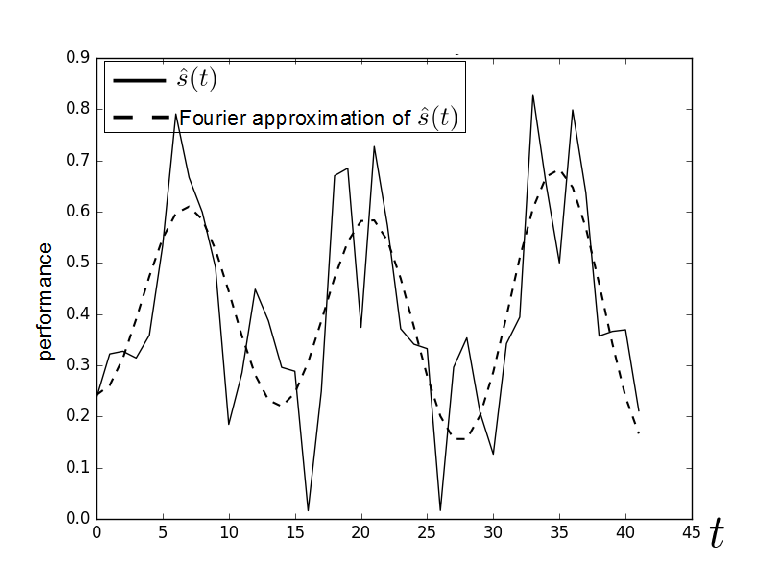
\includegraphics[width=10cm]{contents/chapter-1/sample-fig.png}
	\caption{Contoh gambar.}
	\label{Fig: Contoh gambar}
\end{figure}

Contoh gambar terlihat pada Gambar \ref{Fig: Contoh gambar}. Gambar diambil dari \cite{wibowo2016clustering}.

\subsection{Penulisan Tabel}
\begin{table}[h]
	\caption{Tabel ini}
	\vspace{0.5em}
	\centering
	\begin{tabular}{|c|c|c|}
		\hline
		ID & Tinggi Badan (cm) & Berat Badan (kg) \\
		\hline \hline
		A23 & 173 & 62 \\
		A25 & 185 & 78 \\
		A10 & 162 & 70 \\ \hline
	\end{tabular}
	\label{Tab: Tabel Tinggi Berat}
\end{table}
Contoh penulisan tabel bisa dilihat pada Tabel \ref{Tab: Tabel Tinggi Berat}.

\subsection{Penulisan formula}
Contoh penulisan formula
\begin{equation}
	L_{\psi_z} = \{ t_i \mid v_z(t_i) \le \psi_z \}
\end{equation}

Contoh penulisan secara \textit{inline}: $\mathit{PV = nRT}$. Untuk kasus-kasus tertentu, kita membutuhkan perintah "mathit" dalam penulisan formula untuk menghindari adanya jeda saat penulisan formula.

Contoh formula \textbf{tanpa} menggunakan "mathit": $PVA = RTD$

Contoh formula \textbf{dengan} menggunakan "mathit": $\mathit{PVA = RTD}$



\subsection{Contoh list}
Berikut contoh penggunaan list
\begin{enumerate}
	\item First item
	\item Second item
	\item Third item
\end{enumerate}

\section{Blok Beda Halaman}

\subsection{Membuat algoritma terpisah}

Untuk membuat algoritma terpisah seperti pada contoh berikut, kita dapat memanfaatkan perintah \textit{algstore} dan \textit{algrestore} yang terdapat pada paket \textit{algcompatible}. Pada dasarnya, kita membuat dua blok algoritma dimana blok pertama kita simpan menggunakan \textit{algstore} dan kemudian di-restore menggunakan \textit{algrestore} pada algoritma kedua. Perintah tersebut dimaksudkan agar terdapat kesinamungan antara kedua blok yang sejatinya adalah satu blok. 

\begin{algorithm}                     
	\caption{Contoh algorima}          
	\label{findme}                          
	\begin{algorithmic} [1]                   
		\Procedure{CreateSet}{$v$}
		\State Create new set containing $v$
		\EndProcedure
		\algstore{myalg}
	\end{algorithmic}
\end{algorithm}

Pada blok algoritma kedua, tidak perlu ditambahkan caption dan label, karena sudah menjadi satu bagian dalam blok pertama. Pembagian algoritma menjadi dua bagian ini berguna jika kita ingin menjelaskan bagian-bagian dari sebuah algoritma, maupun untuk memisah algoritma panjang dalam beberapa halaman.

\begin{algorithm}                     
	\begin{algorithmic} [1]                   
		\algrestore{myalg}
		\Procedure{ConcatSet}{$v$}
		\State Create new set containing $v$
		\EndProcedure
	\end{algorithmic}
\end{algorithm}


\subsection{Membuat tabel terpisah}

Untuk membuat tabel panjang yang melebihi satu halaman, kita dapat mengganti kombinasi \textit{table + tabular} menjadi \textit{longtable} dengan contoh sebagai berikut.

\begin{longtable}{| c | c |} 
	\caption{Contoh tabel panjang}
	\label{tab:myfirstlongtable} \\
	\hline
	header 1 & header 2 \\
	\hline \hline
	foo & bar \\ \hline 
	foo & bar \\ \hline
	foo & bar \\ \hline
	foo & bar \\ \hline
	foo & bar \\ \hline
	foo & bar \\ \hline
	foo & bar \\ \hline
	foo & bar \\ \hline
	foo & bar \\ \hline
	foo & bar \\ \hline
	foo & bar \\ \hline
\end{longtable}


\subsection{Menulis formula terpisah halaman}

Terkadang kita butuh untuk menuliskan rangkaian formula dalam jumlah besar sehingga melewati batas satu halaman. Solusi yang digunakan bisa saja dengan memindahkan satu blok formula tersebut pada halaman yang baru atau memisah rangkaian formula menjadi dua bagian untuk masing-masing halaman. Cara yang pertama mungkin akan menghasilkan alur yang berbeda karena ruang kosong pada halaman pertama akan diisi oleh teks selanjutnya. Sehingga di sini kita dapat memanfaatkan \textit{align} yang sudah diatur dengan mode \textit{allowdisplaybreaks}. Penggunakan \textit{align} ini memungkinkan satu rangkaian formula terpisah berbeda halaman. 

Contoh sederhana dapat digambarkan sebagai berikut.

\begin{align*}
	x &= y^2\\
	x &= y^3\\
	a + b &= c\\
	x &= y - 2\\
	a + b &= d + e \tag{\stepcounter{equation}\theequation}\\
	x^2 + 3 &= y\\
	a(x) &= 2x\\
	b_i &= 5x\\
	10x^2 &= 9x\\
	2x^2 + 3x + 2 &= 0\\
	5x - 2 &= 0\\
	d &= \log x\\
	y &= \sin x
\end{align*}



%======================================

%======================================
%  References
%======================================
\thereferences
% You can change 
%    the filename and location of the files inputted
\bibliography{references}

%Hapus bagian di bawah setelah tidak diperlukan
%\begin{center}
%	\textcolor{red}{
%	Catatan: Daftar pustaka adalah apa yang dirujuk atau disitasi, bukan apa yang telah dibaca, jika tidak ada dalam sitasi maka tidak perlu dituliskan dalam daftar pustaka.}
%\end{center}

%======================================

%======================================
%  Appendix
%======================================
% You can change 
%    the filename and location of the files inputted
%    use \chapterappendix for the first page of the appendix
%    use \chapterappendixadd for the next page

\appendix


\chapterappendix{contents/appendix/appendix-isi-lampiran}
\chapterappendixadd{contents/appendix/appendix-latex}
\chapterappendixadd{contents/appendix/appendix-penulisan-referensi}
\chapterappendixadd{contents/appendix/appendix-code}



%======================================

\end{document}